
%% bare_conf.tex
%% V1.3
%% 2007/01/11
%% by Michael Shell
%% See:
%% http://www.michaelshell.org/
%% for current contact information.
%%
%% This is a skeleton file demonstrating the use of IEEEtran.cls
%% (requires IEEEtran.cls version 1.7 or later) with an IEEE conference paper.
%%
%% Support sites:
%% http://www.michaelshell.org/tex/ieeetran/
%% http://www.ctan.org/tex-archive/macros/latex/contrib/IEEEtran/
%% and
%% http://www.ieee.org/

%%*************************************************************************
%% Legal Notice:
%% This code is offered as-is without any warranty either expressed or
%% implied; without even the implied warranty of MERCHANTABILITY or
%% FITNESS FOR A PARTICULAR PURPOSE! 
%% User assumes all risk.
%% In no event shall IEEE or any contributor to this code be liable for
%% any damages or losses, including, but not limited to, incidental,
%% consequential, or any other damages, resulting from the use or misuse
%% of any information contained here.
%%
%% All comments are the opinions of their respective authors and are not
%% necessarily endorsed by the IEEE.
%%
%% This work is distributed under the LaTeX Project Public License (LPPL)
%% ( http://www.latex-project.org/ ) version 1.3, and may be freely used,
%% distributed and modified. A copy of the LPPL, version 1.3, is included
%% in the base LaTeX documentation of all distributions of LaTeX released
%% 2003/12/01 or later.
%% Retain all contribution notices and credits.
%% ** Modified files should be clearly indicated as such, including  **
%% ** renaming them and changing author support contact information. **
%%
%% File list of work: IEEEtran.cls, IEEEtran_HOWTO.pdf, bare_adv.tex,
%%                    bare_conf.tex, bare_jrnl.tex, bare_jrnl_compsoc.tex
%%*************************************************************************

% *** Authors should verify (and, if needed, correct) their LaTeX system  ***
% *** with the testflow diagnostic prior to trusting their LaTeX platform ***
% *** with production work. IEEE's font choices can trigger bugs that do  ***
% *** not appear when using other class files.                            ***
% The testflow support page is at:
% http://www.michaelshell.org/tex/testflow/



% Note that the a4paper option is mainly intended so that authors in
% countries using A4 can easily print to A4 and see how their papers will
% look in print - the typesetting of the document will not typically be
% affected with changes in paper size (but the bottom and side margins will).
% Use the testflow package mentioned above to verify correct handling of
% both paper sizes by the user's LaTeX system.
%
% Also note that the "draftcls" or "draftclsnofoot", not "draft", option
% should be used if it is desired that the figures are to be displayed in
% draft mode.
%
\documentclass[conference]{IEEEtran}
% Add the compsoc option for Computer Society conferences.
%
% If IEEEtran.cls has not been installed into the LaTeX system files,
% manually specify the path to it like:
% \documentclass[conference]{../sty/IEEEtran}





% Some very useful LaTeX packages include:
% (uncomment the ones you want to load)


% *** MISC UTILITY PACKAGES ***
%
%\usepackage{ifpdf}
% Heiko Oberdiek's ifpdf.sty is very useful if you need conditional
% compilation based on whether the output is pdf or dvi.
% usage:
% \ifpdf
%   % pdf code
% \else
%   % dvi code
% \fi
% The latest version of ifpdf.sty can be obtained from:
% http://www.ctan.org/tex-archive/macros/latex/contrib/oberdiek/
% Also, note that IEEEtran.cls V1.7 and later provides a builtin
% \ifCLASSINFOpdf conditional that works the same way.
% When switching from latex to pdflatex and vice-versa, the compiler may
% have to be run twice to clear warning/error messages.






% *** CITATION PACKAGES ***
%
%\usepackage{cite}
% cite.sty was written by Donald Arseneau
% V1.6 and later of IEEEtran pre-defines the format of the cite.sty package
% \cite{} output to follow that of IEEE. Loading the cite package will
% result in citation numbers being automatically sorted and properly
% "compressed/ranged". e.g., [1], [9], [2], [7], [5], [6] without using
% cite.sty will become [1], [2], [5]--[7], [9] using cite.sty. cite.sty's
% \cite will automatically add leading space, if needed. Use cite.sty's
% noadjust option (cite.sty V3.8 and later) if you want to turn this off.
% cite.sty is already installed on most LaTeX systems. Be sure and use
% version 4.0 (2003-05-27) and later if using hyperref.sty. cite.sty does
% not currently provide for hyperlinked citations.
% The latest version can be obtained at:
% http://www.ctan.org/tex-archive/macros/latex/contrib/cite/
% The documentation is contained in the cite.sty file itself.






% *** GRAPHICS RELATED PACKAGES ***
%
\ifCLASSINFOpdf
  % \usepackage[pdftex]{graphicx}
  % declare the path(s) where your graphic files are
  % \graphicspath{{../pdf/}{../jpeg/}}
  % and their extensions so you won't have to specify these with
  % every instance of \includegraphics
  % \DeclareGraphicsExtensions{.pdf,.jpeg,.png}
\else
  % or other class option (dvipsone, dvipdf, if not using dvips). graphicx
  % will default to the driver specified in the system graphics.cfg if no
  % driver is specified.
  % \usepackage[dvips]{graphicx}
  % declare the path(s) where your graphic files are
  % \graphicspath{{../eps/}}
  % and their extensions so you won't have to specify these with
  % every instance of \includegraphics
  % \DeclareGraphicsExtensions{.eps}
\fi
% graphicx was written by David Carlisle and Sebastian Rahtz. It is
% required if you want graphics, photos, etc. graphicx.sty is already
% installed on most LaTeX systems. The latest version and documentation can
% be obtained at: 
% http://www.ctan.org/tex-archive/macros/latex/required/graphics/
% Another good source of documentation is "Using Imported Graphics in
% LaTeX2e" by Keith Reckdahl which can be found as epslatex.ps or
% epslatex.pdf at: http://www.ctan.org/tex-archive/info/
%
% latex, and pdflatex in dvi mode, support graphics in encapsulated
% postscript (.eps) format. pdflatex in pdf mode supports graphics
% in .pdf, .jpeg, .png and .mps (metapost) formats. Users should ensure
% that all non-photo figures use a vector format (.eps, .pdf, .mps) and
% not a bitmapped formats (.jpeg, .png). IEEE frowns on bitmapped formats
% which can result in "jaggedy"/blurry rendering of lines and letters as
% well as large increases in file sizes.
%
% You can find documentation about the pdfTeX application at:
% http://www.tug.org/applications/pdftex





% *** MATH PACKAGES ***
%
%\usepackage[cmex10]{amsmath}
% A popular package from the American Mathematical Society that provides
% many useful and powerful commands for dealing with mathematics. If using
% it, be sure to load this package with the cmex10 option to ensure that
% only type 1 fonts will utilized at all point sizes. Without this option,
% it is possible that some math symbols, particularly those within
% footnotes, will be rendered in bitmap form which will result in a
% document that can not be IEEE Xplore compliant!
%
% Also, note that the amsmath package sets \interdisplaylinepenalty to 10000
% thus preventing page breaks from occurring within multiline equations. Use:
%\interdisplaylinepenalty=2500
% after loading amsmath to restore such page breaks as IEEEtran.cls normally
% does. amsmath.sty is already installed on most LaTeX systems. The latest
% version and documentation can be obtained at:
% http://www.ctan.org/tex-archive/macros/latex/required/amslatex/math/





% *** SPECIALIZED LIST PACKAGES ***
%
%\usepackage{algorithmic}
% algorithmic.sty was written by Peter Williams and Rogerio Brito.
% This package provides an algorithmic environment fo describing algorithms.
% You can use the algorithmic environment in-text or within a figure
% environment to provide for a floating algorithm. Do NOT use the algorithm
% floating environment provided by algorithm.sty (by the same authors) or
% algorithm2e.sty (by Christophe Fiorio) as IEEE does not use dedicated
% algorithm float types and packages that provide these will not provide
% correct IEEE style captions. The latest version and documentation of
% algorithmic.sty can be obtained at:
% http://www.ctan.org/tex-archive/macros/latex/contrib/algorithms/
% There is also a support site at:
% http://algorithms.berlios.de/index.html
% Also of interest may be the (relatively newer and more customizable)
% algorithmicx.sty package by Szasz Janos:
% http://www.ctan.org/tex-archive/macros/latex/contrib/algorithmicx/




% *** ALIGNMENT PACKAGES ***
%
%\usepackage{array}
% Frank Mittelbach's and David Carlisle's array.sty patches and improves
% the standard LaTeX2e array and tabular environments to provide better
% appearance and additional user controls. As the default LaTeX2e table
% generation code is lacking to the point of almost being broken with
% respect to the quality of the end results, all users are strongly
% advised to use an enhanced (at the very least that provided by array.sty)
% set of table tools. array.sty is already installed on most systems. The
% latest version and documentation can be obtained at:
% http://www.ctan.org/tex-archive/macros/latex/required/tools/


%\usepackage{mdwmath}
%\usepackage{mdwtab}
% Also highly recommended is Mark Wooding's extremely powerful MDW tools,
% especially mdwmath.sty and mdwtab.sty which are used to format equations
% and tables, respectively. The MDWtools set is already installed on most
% LaTeX systems. The lastest version and documentation is available at:
% http://www.ctan.org/tex-archive/macros/latex/contrib/mdwtools/


% IEEEtran contains the IEEEeqnarray family of commands that can be used to
% generate multiline equations as well as matrices, tables, etc., of high
% quality.


%\usepackage{eqparbox}
% Also of notable interest is Scott Pakin's eqparbox package for creating
% (automatically sized) equal width boxes - aka "natural width parboxes".
% Available at:
% http://www.ctan.org/tex-archive/macros/latex/contrib/eqparbox/





% *** SUBFIGURE PACKAGES ***
%\usepackage[tight,footnotesize]{subfigure}
% subfigure.sty was written by Steven Douglas Cochran. This package makes it
% easy to put subfigures in your figures. e.g., "Figure 1a and 1b". For IEEE
% work, it is a good idea to load it with the tight package option to reduce
% the amount of white space around the subfigures. subfigure.sty is already
% installed on most LaTeX systems. The latest version and documentation can
% be obtained at:
% http://www.ctan.org/tex-archive/obsolete/macros/latex/contrib/subfigure/
% subfigure.sty has been superceeded by subfig.sty.



%\usepackage[caption=false]{caption}
%\usepackage[font=footnotesize]{subfig}
% subfig.sty, also written by Steven Douglas Cochran, is the modern
% replacement for subfigure.sty. However, subfig.sty requires and
% automatically loads Axel Sommerfeldt's caption.sty which will override
% IEEEtran.cls handling of captions and this will result in nonIEEE style
% figure/table captions. To prevent this problem, be sure and preload
% caption.sty with its "caption=false" package option. This is will preserve
% IEEEtran.cls handing of captions. Version 1.3 (2005/06/28) and later 
% (recommended due to many improvements over 1.2) of subfig.sty supports
% the caption=false option directly:
%\usepackage[caption=false,font=footnotesize]{subfig}
%
% The latest version and documentation can be obtained at:
% http://www.ctan.org/tex-archive/macros/latex/contrib/subfig/
% The latest version and documentation of caption.sty can be obtained at:
% http://www.ctan.org/tex-archive/macros/latex/contrib/caption/




% *** FLOAT PACKAGES ***
%
%\usepackage{fixltx2e}
% fixltx2e, the successor to the earlier fix2col.sty, was written by
% Frank Mittelbach and David Carlisle. This package corrects a few problems
% in the LaTeX2e kernel, the most notable of which is that in current
% LaTeX2e releases, the ordering of single and double column floats is not
% guaranteed to be preserved. Thus, an unpatched LaTeX2e can allow a
% single column figure to be placed prior to an earlier double column
% figure. The latest version and documentation can be found at:
% http://www.ctan.org/tex-archive/macros/latex/base/



%\usepackage{stfloats}
% stfloats.sty was written by Sigitas Tolusis. This package gives LaTeX2e
% the ability to do double column floats at the bottom of the page as well
% as the top. (e.g., "\begin{figure*}[!b]" is not normally possible in
% LaTeX2e). It also provides a command:
%\fnbelowfloat
% to enable the placement of footnotes below bottom floats (the standard
% LaTeX2e kernel puts them above bottom floats). This is an invasive package
% which rewrites many portions of the LaTeX2e float routines. It may not work
% with other packages that modify the LaTeX2e float routines. The latest
% version and documentation can be obtained at:
% http://www.ctan.org/tex-archive/macros/latex/contrib/sttools/
% Documentation is contained in the stfloats.sty comments as well as in the
% presfull.pdf file. Do not use the stfloats baselinefloat ability as IEEE
% does not allow \baselineskip to stretch. Authors submitting work to the
% IEEE should note that IEEE rarely uses double column equations and
% that authors should try to avoid such use. Do not be tempted to use the
% cuted.sty or midfloat.sty packages (also by Sigitas Tolusis) as IEEE does
% not format its papers in such ways.





% *** PDF, URL AND HYPERLINK PACKAGES ***
%
%\usepackage{url}
% url.sty was written by Donald Arseneau. It provides better support for
% handling and breaking URLs. url.sty is already installed on most LaTeX
% systems. The latest version can be obtained at:
% http://www.ctan.org/tex-archive/macros/latex/contrib/misc/
% Read the url.sty source comments for usage information. Basically,
% \url{my_url_here}.



\usepackage{amssymb}
\usepackage{url}
\usepackage{amsmath}
\usepackage{amsthm}
\usepackage{graphicx}

\usepackage[boxed,noline]{algorithm2e}
\usepackage{relsize}
%\pagestyle{headings}

\newcommand{\hide}[1]{}
\newcommand{\eg}{{\em e.g.}}
\newcommand{\ie}{{\em i.e.}}

\theoremstyle{plain}
\newtheorem{proposition}{Proposition}

\theoremstyle{definition}
\newtheorem{definition}{Definition}
\newtheorem{example}{Example}

\theoremstyle{remark}
\newtheorem*{remark}{Remark}



% correct bad hyphenation here
\hyphenation{op-tical net-works semi-conduc-tor}


\begin{document}
%
% paper title
% can use linebreaks \\ within to get better formatting as desired
\title{Verification of probabilistic bounded $\delta$-reachability for cyber-physical systems}


% author names and affiliations
% use a multiple column layout for up to three different
% affiliations
\author{\IEEEauthorblockN{Fedor Shmarov}
\IEEEauthorblockA{School of Computing Science, Newcastle University\\
Newcastle, NE1 7RU, UK\\
Email: f.shmarov@ncl.ac.uk}
\and
\IEEEauthorblockN{Paolo Zuliani}
\IEEEauthorblockA{School of Computing Science, Newcastle University\\
Newcastle, NE1 7RU, UK\\
Email: paolo.zuliani@ncl.ac.uk}
}

% conference papers do not typically use \thanks and this command
% is locked out in conference mode. If really needed, such as for
% the acknowledgment of grants, issue a \IEEEoverridecommandlockouts
% after \documentclass

% for over three affiliations, or if they all won't fit within the width
% of the page, use this alternative format:
% 
%\author{\IEEEauthorblockN{Michael Shell\IEEEauthorrefmark{1},
%Homer Simpson\IEEEauthorrefmark{2},
%James Kirk\IEEEauthorrefmark{3}, 
%Montgomery Scott\IEEEauthorrefmark{3} and
%Eldon Tyrell\IEEEauthorrefmark{4}}
%\IEEEauthorblockA{\IEEEauthorrefmark{1}School of Electrical and Computer Engineering\\
%Georgia Institute of Technology,
%Atlanta, Georgia 30332--0250\\ Email: see http://www.michaelshell.org/contact.html}
%\IEEEauthorblockA{\IEEEauthorrefmark{2}Twentieth Century Fox, Springfield, USA\\
%Email: homer@thesimpsons.com}
%\IEEEauthorblockA{\IEEEauthorrefmark{3}Starfleet Academy, San Francisco, California 96678-2391\\
%Telephone: (800) 555--1212, Fax: (888) 555--1212}
%\IEEEauthorblockA{\IEEEauthorrefmark{4}Tyrell Inc., 123 Replicant Street, Los Angeles, California 90210--4321}}



% make the title area
\maketitle


\begin{abstract}
%\boldmath
Verification of cyber-physical systems is a difficult, yet extremely important, problem. 
Hybrid systems offer a theoretical framework in which to perform formal verification of
cyber-physical systems.
In this paper we study the problem of bounded $\delta$-reachability in hybrid systems with random 
initial parameters. We devise a technique for computing reachability 
probabilities over a finite number of discrete steps for nonlinear
hybrid systems featuring a bounded random initial parameter.
Our approach is to define an appropriate $\delta$-relaxation 
of the (undecidable) reachability problem, so that it can be solved by a $\delta$-complete 
decision procedure. Specifically, we can compute an interval that is guaranteed to contain 
the probability of, say, a hybrid system behaving in a faulty way. Moreover, we discuss 
certain types of random variables with unbounded support and show that the bounded 
$\delta$-reachability problem can still be solved by using an appropriate $\delta$-complete
decision procedure. Finally, we propose the development of a validated integration procedure 
over an arbitrary Borel set in order to cope with hybrid systems with dynamics given by
solutions of ordinary differential equations.
\end{abstract}
% IEEEtran.cls defaults to using nonbold math in the Abstract.
% This preserves the distinction between vectors and scalars. However,
% if the conference you are submitting to favors bold math in the abstract,
% then you can use LaTeX's standard command \boldmath at the very start
% of the abstract to achieve this. Many IEEE journals/conferences frown on
% math in the abstract anyway.

% no keywords




% For peer review papers, you can put extra information on the cover
% page as needed:
% \ifCLASSOPTIONpeerreview
% \begin{center} \bfseries EDICS Category: 3-BBND \end{center}
% \fi
%
% For peerreview papers, this IEEEtran command inserts a page break and
% creates the second title. It will be ignored for other modes.
\IEEEpeerreviewmaketitle



\section{Introduction}
\section{Introduction}\label{sec:intro}

% Need a paragrapgh or two to explain why the tool is interesting and
% significant should be provided.

\dReach{} is a bounded reachability analysis tool for hybrid systems.
It encodes bounded reachability problems of hybrid systems as
first-order formulas over the real numbers, and solves them using
$\delta$-decision procedures in the SMT solver
\dReal{}~\cite{DBLP:conf/cade/GaoKC13}. \dReach{} is able to handle a
wide range of highly nonlinear hybrid systems~\cite{CMSB14,DBLP:conf/fmcad/GaoKC13,DBLP:conf/hybrid/KapinskiDSA14,6868816}.
Figure~\ref{fig:prostate-example} highlights some of its features: on
the left is an example of some nonlinear dynamics that \dReach{} can
handle, and on the right a visualized counterexample generated by
\dReach{} on this model.
\begin{figure}[!h]
  \subfloat[An example of nonlinear hybrid system model: off-treatment
  mode of the prostate cancer treatment model~\cite{CMSB14}\label{subfig-1:prostate}]{
    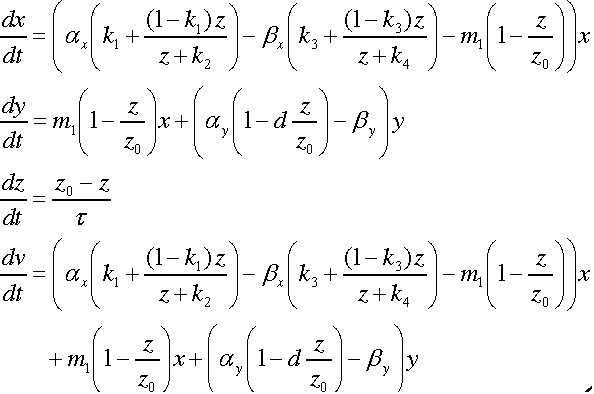
\includegraphics[width=0.45\textwidth]{images/prostatebw-mode2.pdf}
  }
  \hfill
  \subfloat[Visualization of a generated counterexample. Change in the shade of colors represents discrete mode changes.]{%
    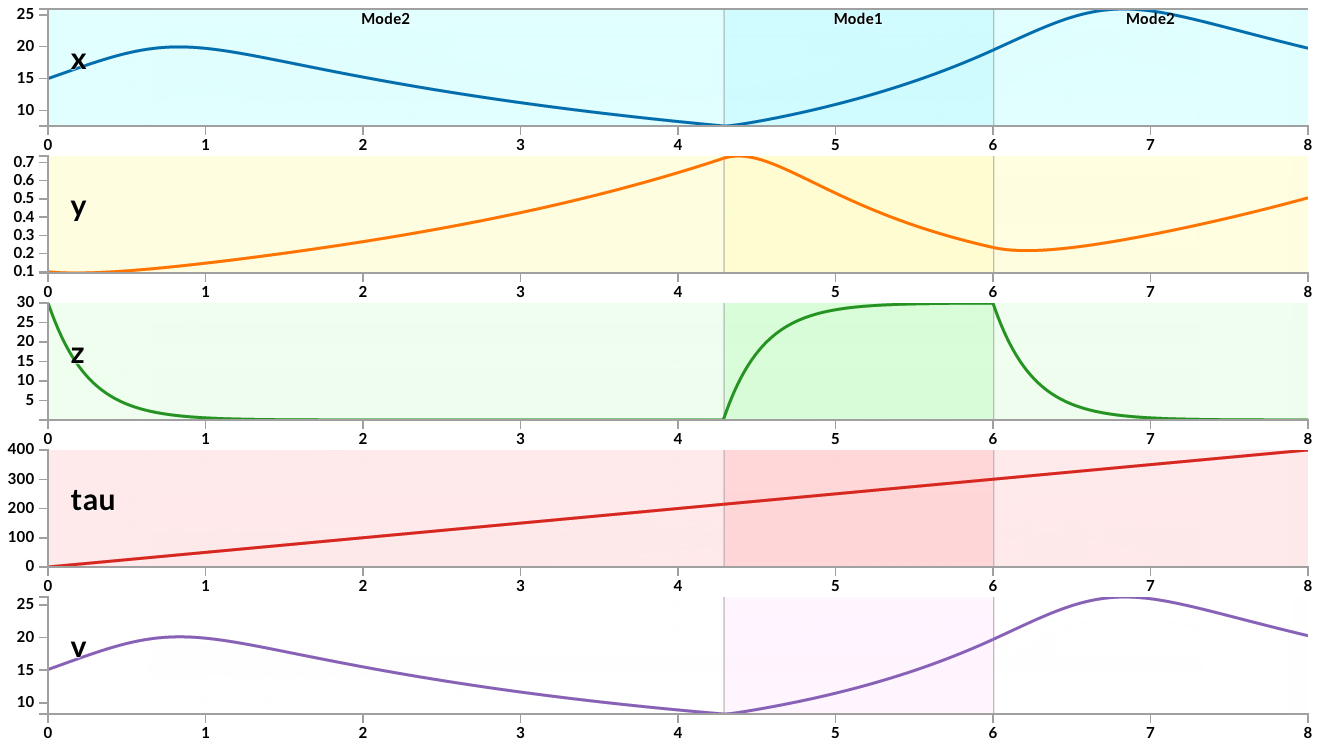
\includegraphics[width=0.48\textwidth]{images/prostate}
  }
  \caption{An example of nonlinear dynamics and counterexample-generation.}
  \label{fig:prostate-example}
\end{figure}

It is well-known that the standard bounded reachability problems for
simple hybrid systems are already highly
undecidable~\cite{DBLP:conf/hybrid/AlurCHH92}.
Instead, we work in the framework of $\delta$-reachability of hybrid systems~\cite{DBLP:journals/corr/GaoKCC14}.
Here $\delta$ is an arbitrary positive rational number, provided by the user to
specify the bound on numerical errors that can be tolerated in the analysis.
For a hybrid system $H$ and an unsafe region $\unsafe$ (both encoded as logic formulas),
the $\delta$-reachability problem asks for one of the following answers:
\begin{itemize}
        \item {\sf safe}: $H$ cannot reach $\unsafe$.
        \item {\sf $\delta$-unsafe}: $H^{\delta}$ can reach $\unsafe^{\delta}$.
\end{itemize}
Here, $H^{\delta}$ and $\unsafe^{\delta}$ encode ($\delta$-bounded) overapproximations
of $H$ and $\unsafe$, defined explicitly as their syntactic variants.%(See Section~\ref{sec:delta-reachability} in the Appendix.)
It is important to note that the definition makes the answers no weaker than standard reachability:
When {\sf safe} is the answer, we know for certain that $H$ does not reach
the unsafe region (no $\delta$ is involved); when {\sf $\delta$-unsafe} is the answer,
we know that there exists some $\delta$-bounded perturbation of the system that can render it unsafe.
Since $\delta$ can be chosen to be very small, {\sf$\delta$-unsafe} answers in fact
discover robustness problem in the system, which should be regarded as unsafe indeed.
We have proved that bounded $\delta$-reachabilty is decidable for a wide range
of nonlinear hybrid systems, even with reasonable complexity bounds~\cite{DBLP:journals/corr/GaoKCC14}.
This framework provides the formal correctness guarantees of \dReach{}.

Apart from solving $\delta$-reachability, the following key features of \dReach{}
distinguish it from other existing tools in this
domain~\cite{DBLP:journals/jlp/FranzleTE10,DBLP:conf/cav/FrehseGDCRLRGDM11,DBLP:journals/tac/AlthoffK14,DBLP:conf/hybrid/Frehse05,DBLP:conf/icons/HerdeEFT08,DBLP:conf/rtss/ChenAS12,DBLP:conf/aaai/CimattiMT12}.
%insert explanations for each item.
\begin{enumerate}
\item Expressiveness. \dReach{} allows the user to describe hybrid
  systems using first-order logic formulas over real numbers with a
  wide range of nonlinear functions. This allows the user to specify
  the continuous flows using highly nonlinear differential equations,
  and the jump and reset conditions with complex Boolean combinations
  of nonlinear constraints. \dReach{} also faithfully translates mode
  invariants into $\exists\forall$ logic formulas, which can be
  directly solved under certain restrictions on the invariants.
\item Property-guided search. \dReach{} maintains logical encodings
  (the same approach as~\cite{DBLP:conf/aaai/CimattiMT12}), whose size
  is linear in the size of the inputs, of the reachable states of a
  hybrid system~\cite{DBLP:journals/corr/GaoKCC14}. The tool searches
  for concrete counterexamples to falsify the reachability properties,
  instead of overapproximating the full reachable states. This avoids
  the usual state explosion problem in reachable set computation,
  because the full set of states does not need to be explicitly
  stored. This change is analogous to the difference between SAT-based
  model checking and BDD-based symbolic model checking.
\item Tight integration of symbolic reasoning and numerical solving.
  \dReach{} delegates the reasoning on discrete mode changes to SAT
  solvers, and uses numerical constraint solving to handle nonlinear
  dynamics. As a result, it can combine the full power of both
  symbolic reasoning and numerical analysis algorithms. In particular,
  all existing tools for reachable set computation can be easily
  plugged-in as engines for solving the continuous part of the
  dynamics, while logic reasoning tools can overcome the difficulty in
  handling complex mode transitions.
\end{enumerate}
The paper is structured as follows. We describe the system architecture in Section 2,
and give some details about the logical encoding in the tool in Section 3.
We then explain the input format and usage in Section 4. %More details and examples are given in the Appendix.

%Realistic hybrid systems involves nonlinear ODEs with transcendental
%functions. \dReach{} allows users to specify a hybrid system in a
%nonlinear signature as it is without linearizing or overapproximating
%it. Users can provide the tool with a numerical error bound $\delta$,
%a bounded time horizon $[0, T]$, and a maximum number of mode switches
%$k$ for the analysis. As a result of analysis, \dReach{} will return
%either \textbf{$\delta$-sat} with a concrete counterexample, or
%\textbf{unsat} which does not involve numerical errors. We also
%provide a visualization for the $\delta$-sat case to help
%understand the analysis result.

% TODO: Need to differentiate this paper from FMCAD paper
%  - FMCAD: underlying solving techniques for SMT with ODEs
%  - TACAS: tool, encoding, using solver...

%%% Local Variables:
%%% mode: latex
%%% TeX-master: "main"
%%% End:


\section{Bounded $\delta$-Reachability in Hybrid Systems}

We now formally define hybrid systems, which we use for modelling cyber-physical systems. The following
definition is standard.

\begin{definition}
A hybrid system consists of the following components:
\begin{itemize}
\item $Q = \{q_0, ..., q_m\}$ a set of modes (discrete components of the system),
\item $X = [u_1, v_1] \times ... \times [u_n, v_n] \times [0, T] \subset \mathbb{R}^{n+1}$ a domain 
	of continuous variables,
\item $S = Q \times X$ is the hybrid state space of the system,
\item $U \subseteq S$ an {\em unsafe} region of the state space,
\end{itemize}
and predicates (or relations)
\begin{itemize}
	\item $\text{flow}_{q}(\textbf{x}^{0}, \textbf{x}^{t})$ mapping the continuous state 
	$\textbf{x}^{0}$ at time 0 to state $\textbf{x}^{t}$ at time point $t \in [0, T]$ in mode $q$
	\item $\text{init}_q(\textbf{x})$ indicating that $s = (q, \textbf{x})$ belongs to the set 
	of initial states,
	\item $\text{jump}_{q \rightarrow q'}(\textbf{x}^{t}, \textbf{x}^{0})$ indicating that the 
	system can make a transition from mode $q$, upon reaching the jump condition in continuous 
	state $\textbf{x}^{t}$ at time point $t \in [0, T]$, to mode $q^\prime$ and setting the
	continuous state to $\textbf{x}^{0}$,
	\item $\text{unsafe}_{q}(\textbf{x})$ indicating that $s = (q, \textbf{x}) \in U$
\end{itemize}
\end{definition}
\begin{remark}
The continuous dynamics of the system is defined in each flow, and it can either be presented 
as a system of ODEs or explicitly.
\end{remark}

In this paper we are interested in {\em deterministic} hybrid systems, where in each mode only
one jump is allowed. Informally, the semantics of a hybrid system can be thought as piece-wise
continuous: in each mode the system dynamics follows a continuous flow, while a mode change
(as result of a jump) might also involve a discontinuous change in the variables $\textbf{x}$.
The evolution of a hybrid system is then obtained by iteratively composing the relations flow and
jump, starting with init --- see Definition \ref{def:reachability} below for an example. More details 
can be found in \cite{DBLP:conf/hybrid/AlurCHH92}.

In order to overcome the undecidability of reasoning about hybrid systems, Gao {\em et al.} recently
defined the concept of $\delta$-satisfiability over the reals \cite{DBLP:conf/lics/GaoAC12}, 
and presented a corresponding $\delta$-complete decision procedure \cite{DBLP:conf/cade/GaoAC12}. 
The main idea is to decide correctly whether slightly {\em relaxed} sentences over the reals 
are satisfiable or not. The following definitions are from \cite{DBLP:conf/lics/GaoAC12}.
\begin{definition}
A bounded quantifier is one of the following:
\[ \begin{array}{ll}
	\exists^{[a, b]} x  = \exists x : (a \le x \wedge x \le b) \\[1ex]
	\forall^{[a, b]} x  = \forall x : (a \le x \wedge x \le b)
\end{array} \]
\end{definition}

\begin{definition}
A bounded $\Sigma_1$ sentence is an expression of the form:
\begin{equation*} 
	\exists^{I_{1}} x_{1}, ..., \exists^{I_{1}} x_{n}: \psi(x_{1}, ..., x_{n})
\end{equation*}
where $I_{i} = [a_{i}, b_{i}]$ are intervals, $\psi(x_{1}, ..., x_{n})$ is a Boolean combination 
of atomic formulas of the form $g(x_{1}, ..., x_{n})\, \texttt{op} \, 0$, where $g$ is a composition 
of Type 2-computable functions and $\texttt{op} \in \{<, \le, >, \ge, =, \ne\}$. 
\end{definition}
\begin{remark}
Any bounded $\Sigma_1$ sentence is equivalent to a $\Sigma_1$ sentence in which all the atoms are
of the form $f(x_{1}, ..., x_{n}) = 0$ (\ie, the only \texttt{op} needed is `=') 
\cite{DBLP:conf/cade/GaoAC12}.
\end{remark}
Essentially, Type 2-computable functions can be approximated arbitrarily well by finite
computations of a special kind of Turing machines (Type 2 machines); most `useful' functions over 
the reals (\eg, continuous functions) are Type 2-computable \cite{kobook}.

The notion of $\delta$-weakening \cite{DBLP:conf/lics/GaoAC12} of a bounded sentence is central
to $\delta$-satisfiability.
\begin{definition}
Let $\delta \in \mathbb{Q^+} \cup \{0\}$ be a constant and $\phi$ a bounded $\Sigma_1$-sentence 
in the standard form 
\begin{equation} \label{def:sigma1}
\phi = \exists^{I_{1}} x_{1}, ..., \exists^{I_{n}} x_{n}: \bigwedge^{m}_{i = 1}(\bigvee^{k_i}_{j = 1} f_{ij}(x_{1}, ..., x_{n}) = 0)
\end{equation}
where $f_{ij}(x_{1}, ..., x_{n}) = 0$ are atomic formulas. The $\delta$-{\em weakening} of $\phi$ 
is the formula:
\begin{equation}
\phi^\delta = \exists^{I_{1}} x_{1}, ..., \exists^{I_{n}} x_{n}: \bigwedge^{m}_{i = 1}(\bigvee^{k_i}_{j = 1} |f_{ij}(x_1, ..., x_n)| \le \delta)
\end{equation}
\end{definition}
Note that $\phi$ implies $\phi^\delta$, while the converse is obviously not true.
The bounded $\delta$-satisfiability problem asks for the following: given a sentence of 
the form (\ref{def:sigma1}) and $\delta \in \mathbb{Q^+}$, correctly decide whether
\begin{itemize}
	\item \textbf{unsat}: $\phi$ is false,
	\item \textbf{$\delta$-true}: $\phi^\delta$ is true.
\end{itemize}
If the two cases overlap either decision can be returned: such a scenario reveals that the 
formula is {\em fragile} --- a small perturbation (\ie, a small $\delta$) can change the formula's
truth value. The dReal tool \cite{DBLP:conf/cade/GaoKC13} implements an algorithm for solving 
the $\delta$-satisfiability problem. Basically, the algorithm combines a DPLL procedure \cite{DPLL} 
(for handling the Boolean parts of the formula) with interval constraint propagation \cite{handbookICP}
(for handling the real arithmetic atoms). More details on the implementation can be found 
in \cite{DBLP:conf/cade/GaoKC13}.

A qualitative property of hybrid systems that can be checked is bounded $\delta$-reachability. 
It asks whether the system reaches the unsafe region after $k \in \mathbb{N}$ discrete transitions.


\begin{definition} \cite{DBLP:journals/corr/GaoKCC14}\label{def:reachability}
Bounded $k$ step $\delta$-reachability in hybrid systems can be encoded as a bounded $\Sigma_1$-sentence
\begin{equation} \label{eq:reachability}
\begin{split}
\exists \textbf{x}^{0}_{0,q_0}, \exists \textbf{x}^{t}_{0,q_0}, ... , \exists \textbf{x}^{0}_{0,q_m}, \exists \textbf{x}^{t}_{0,q_m} , ... , \exists \textbf{x}^{0}_{k,q_m}, \exists \textbf{x}^{t}_{k,q_m}:\\
(\bigvee_{q \in Q} (\text{init}_{q}(\textbf{x}^{0}_{0,q}) \wedge \text{flow}_{q}(\textbf{x}^{0}_{0,q},\textbf{x}^{t}_{0,q}))) \\
\wedge (\bigwedge_{i=0}^{k-1} (\bigvee_{q,q' \in Q}(\text{jump}_{q \rightarrow q'}(\textbf{x}^{t}_{i,q}, \textbf{x}^{0}_{i+1,q'}) \\
\wedge (\text{flow}_{q'}(\textbf{x}^{0}_{i+1,q'}, \textbf{x}^{t}_{i+1,q'}))) \wedge (\bigvee_{q \in Q} \text{unsafe}_{q}(\textbf{x}^{t}_{k,q}))))
\end{split}
\end{equation}
where $\textbf{x}^{0}_{i,q}$ and $\textbf{x}_{i,q}$ represent the continuous state in the mode $q$ at the depth $i$, and $q'$ is a successor mode.
\end{definition}

Intuitively, the formula above can be understood as follows: the first conjunction is asking for 
a set of continuous variables which satisfy the initial condition in one of the modes and the 
flow in that mode; the second conjunction is looking for a set of vectors which satisfy any $k$ 
discrete jumps and flows in each successor mode defined by the jumps; the third conjunction is 
verifying whether the state of the system (the mode and the set of continuous variables in the 
mode after $k$ jumps) belongs to the unsafe region. Note that the previous definition asks for
reachability in {\em exactly} $k$ steps. One can build a disjunction of formula (\ref{eq:reachability})
for all values from 1 to $k$, thereby obtaining reachability {\em within} $k$ steps.

The $\delta$-reachability problem can be solved using the described $\delta$-complete decision 
procedure, which will correctly return one of the following answers: 
\begin{itemize}
	\item \textbf{unsat}: the system never reaches the bad region $U$,
	\item \textbf{$\delta$-true}: the $\delta$-perturbation of (\ref{eq:reachability}) is true,
	and a witness, \ie, an assignment for all the variables, is returned.
\end{itemize}




\section{Bounded $\delta$-Reachability in Probabilistic Hybrid Systems}
We now introduce $\delta$-reachability in a probabilistic context.

\begin{definition}\label{def:pHS}
A hybrid system with {\em random initial parameters} consists of the following components:
\begin{itemize}
\item $Q = \{q_0, ..., q_m\}$ a set of modes (discrete components of the system),
\item $X = [u_1, v_1] \times ... \times [u_n, v_n] \times [0, T] \subset \mathbb{R}^{n+1}$ a domain 
	of continuous variables,
\item $R = [a_1, b_1] \times ... \times [a_l, b_l] \subset \mathbb{R}^{l}$ a domain of {\em random}
	parameters,
\item $S = Q \times R \times X$ is the state space of the system,
\item $U \subseteq S$ an {\em unsafe} region of the state space,
\end{itemize}
predicates (relations)
\begin{itemize}
	\item $\text{flow}_{q}(\textbf{r}, \textbf{x}^{0}, \textbf{x}^{t})$ mapping the continuous state 
	$\textbf{x}^{0}$ at time 0 to state $\textbf{x}^{t}$ at time point $t \in [0, T]$ in mode $q$
	\item $\text{init}_q(\textbf{r}, \textbf{x})$ indicating that $ (q, \textbf{r}, \textbf{x})$ 
	belongs to the set of initial states,
	\item $\text{jump}_{q \rightarrow q'}(\textbf{r}, \textbf{x}^{t}, \textbf{x}^{0})$ indicating that the 
	system can make a transition from mode $q$, upon reaching the jump condition in continuous 
	state $\textbf{x}^{t}$ at time point $t \in [0, T]$, to mode $q^\prime$ and setting the
	continuous state to $\textbf{x}^{0}$,
	\item $\text{unsafe}_{q}(\textbf{r}, \textbf{x})$ indicating that 
	$(q, \textbf{r}, \textbf{x}) \in U$,
\end{itemize}
and we require that for all $q\in Q$ the sets defined by $\text{flow}_q, \text{init}_q, \text{jump}_q$,
and $\text{unsafe}_q$ are Borel.
\end{definition}
\begin{remark}
The newly introduced random parameters are assigned in the initial mode and remain unchanged throughout
the system's evolution: note that flow and jump do not specify any change on $\textbf{r}$. Also, the
Borel assumption for the sets defined by the predicates is a theoretical requirement for well-definedness
of probabilities, and in practice it is easily satisfied. (We recall that Borel sets are obtained
through countable union and complement of open sets.)
\end{remark}

Then bounded $k$ step reachability problem for the defined system will be modified.
\begin{definition}
The bounded $k$ step $\delta$-reachability for hybrid systems with random initial parameters 
is the $\Sigma_1$ sentence:
\begin{equation*} %\label{eq:reachability-2}
\begin{split}
\exists \textbf{r}, \exists \textbf{x}^{0}_{0,q_0}, \exists \textbf{x}^t_{0,q_0}, ... , \exists \textbf{x}^{0}_{0,q_m}, \exists \textbf{x}^t_{0,q_m} , ... , \exists \textbf{x}^{0}_{k,q_m}, \exists \textbf{x}^t_{k,q_m}:\\
(\bigvee_{q \in Q} (\text{init}_{q}(\textbf{r}, \textbf{x}^{0}_{0,q}) \wedge \text{flow}_{q}(\textbf{r}, \textbf{x}^{0}_{0,q},\textbf{x}^t_{0,q}))) \\
\wedge (\bigwedge_{i=0}^{k-1} (\bigvee_{q,q' \in Q}(\text{jump}_{q \rightarrow q'}(\textbf{r}, \textbf{x}^t_{i,q}, \textbf{x}^{0}_{i+1,q'}) \\
\wedge (\text{flow}_{q'}(\textbf{r}, \textbf{x}^{0}_{i+1,q'}, \textbf{x}^t_{i+1,q'}))) \wedge (\bigvee_{q \in Q} \text{unsafe}_{q}(\textbf{r}, \textbf{x}^t_{k,q}))))
\end{split}
\end{equation*}
\end{definition}

If we associate a probability measure to the random parameters, then we can assess {\em quantitative} 
system properties (such as the probability that the system reaches the unsafe region).
In particular, we consider the following problem: 
\textit{what is the probability that a hybrid system with random initial parameters reaches the 
unsafe region in $k$ steps?}

To calculate the probability of reaching the unsafe region, we first need to find the set 
which contains all the values of the random variables satisfying the reachability property 
of a hybrid system. Such a set is constructed as follows:
\begin{equation} \label{def:Borel-set}
\begin{split}
B = \{\textbf{r} : \exists \textbf{x}^{0}_{0,q_0}, \exists \textbf{x}^t_{0,q_0}, ... , \exists \textbf{x}^{0}_{0,q_m}, \exists \textbf{x}^t_{0,q_m} , ... , \exists \textbf{x}^{0}_{k,q_m}, \exists \textbf{x}^t_{k,q_m}\mathord{:}\\
(\bigvee_{q \in Q} (\text{init}_{q}(\textbf{r}, \textbf{x}^{0}_{0,q}) \wedge \text{flow}_{q}(\textbf{r}, \textbf{x}^{0}_{0,q},\textbf{x}^t_{0,q}))) \\
\wedge (\bigwedge_{i=0}^{k-1} (\bigvee_{q,q' \in Q}(\text{jump}_{q \rightarrow q'}(\textbf{r}, \textbf{x}^t_{i,q}, \textbf{x}^{0}_{i+1,q'}) \\
\wedge (\text{flow}_{q'}(\textbf{r}, \textbf{x}^{0}_{i+1,q'}, \textbf{x}^t_{i+1,q'}))) \wedge (\bigvee_{q \in Q} \text{unsafe}_{q}(\textbf{r}, \textbf{x}^t_{k,q}))))\}.
\end{split}
\end{equation}
\begin{proposition}
The set $B$ defined by (\ref{def:Borel-set}) is Borel.
\end{proposition}
\begin{IEEEproof}
Immediate from the fact that (Definition \ref{def:pHS}) the sets defined 
by $\text{flow}_q, \text{init}_q, \text{jump}_q$, and $\text{unsafe}_q$ are Borel, and conjunction and 
disjunctions correspond to set intersection and union, respectively.
\end{IEEEproof}

The proposition entails that the probability that the system reaches the unsafe region is well-defined. 
Such a probability is computed by integrating the probability measure of  the random variables over the 
set (\ref{def:Borel-set}). In particular, we need to compute the following integral
\begin{equation} \label{eq:probabilistic-reachability}
\int_{B} \,dP(\textbf{r})
\end{equation}
where $B$ is the set (\ref{def:Borel-set}) and $P(\textbf{r})$ is a probability measure over 
the random parameters $\textbf{r}$. In case that the random parameters are independent then 
$P(\textbf{r}) = \Pi_{i=1}^{l} P_i(r_{i})$, where $P_i$ is the probability measure of 
parameter $r_i$. For most practical applications, the infinitesimal probability measure 
$dP(\textbf{r})$ is simply given by a (probability) density function.



\section{Systems with one random parameter}
In the scope of this paper we consider hybrid systems with one random initial parameter, and 
we propose an algorithm solving the probabilistic $\delta$-reachability problem for such 
hybrid systems. In a hybrid system with random parameters, the random variable $r$ is defined 
over a bounded interval. However, we will demonstrate that we can correctly evaluate the 
probabilistic reachability problems also for certain types of unbounded random variables.

\begin{proposition} \label{prop:inf}
The probabilistic reachability problem for hybrid systems with a single random parameter 
can be correctly solved by a $\delta$-complete decision procedure if:
\begin{itemize}
	\item the domain of the random parameter is bounded from one side,
	\item the domain of the random parameter is unbounded and its probability density 
		function is symmetric.
\end{itemize}
\end{proposition}
\begin{IEEEproof}
Let's consider the first case when the domain $\Omega$ of the continuous random variable is bounded from one side. The problem when set $B \subseteq \Omega$ is bounded is trivial and probabilistic reachability problem can be solved correctly by the $\delta$-complete procedure.

If $B$ is unbounded then its complement $\Omega/B$ is bounded (because $\Omega$ is bounded from one side and $B \subseteq \Omega$). Set $\Omega/B$ can be constructed by inverting the relation $\text{unsafe}_{q}(\textbf{r},\textbf{x})$. Taking into account that
\begin{equation} \label{eq:total-probability}
\int_{B} \,dP(r) + \int_{\Omega/B} \,dP(r) = \int_{\Omega} \,dP(r) = 1
\end{equation}
probabilistic reachability problem (\ref{eq:probabilistic-reachability}) is equivalent to
\begin{equation} \label{eq:probabilistic-reachability-one-side}
\exists B_1 \subseteq  \Omega/B: 1 - \int_{B_1} \,dP(r) < C
\end{equation}

Therefore, solving two problems (\ref{eq:probabilistic-reachability}) and (\ref{eq:probabilistic-reachability-one-side}) at the same time by the $\delta$-complete decision procedure guaranties that one of them will terminate with the correct result. Knowing one, we can derive another from the equation (\ref{eq:total-probability}).

Let's consider the second case when $\Omega$ is unbounded and the probability density function is symmetric. We can find two disjoint bounded from one side sets $\Omega^{-}, \Omega^{+} \subset \Omega$ such that $\Omega^{-} \cup \Omega^{+} = \Omega$ and $\int_{\Omega^{-}} \,dP(r) = \int_{\Omega^{+}} \,dP(r) = \frac{\int_{\Omega} \,dP(r)}{2} = 0.5$.

Let $B \subseteq \Omega$. We can find two disjoint sets $B^{-}, B^{+} \subset B$ such that $B^{-} \cup B^{+} = B$, $B^{-} \subseteq \Omega^{-}$ and $B^{+} \subseteq \Omega^{+}$. Then problem (\ref{eq:probabilistic-reachability}) is equivalent to:
\begin{equation} \label{eq:probabilistic-reachability-symmetric}
\exists B_{1}^{-} \subseteq  B^{-}, \exists B_{1}^{+} \subseteq  B^{+} : \int_{B_{1}^{-}} \,dP(r) + \int_{B_{1}^{+}} \,dP(r) \ge C
\end{equation}
where for each of the subsets $B^{-}$ and $B^{+}$:
\begin{equation}
\begin{split}
\int_{B^{+}} \,dP(r) + \int_{\Omega^{+}/B^{+}} \,dP(r)  = 0.5 \\
\int_{B^{-}} \,dP(r) + \int_{\Omega^{-}/B^{-}} \,dP(r)  = 0.5
\end{split}
\end{equation}
If either of subsets $B^{-}$ and $B^{+}$ is unbounded then the technique described above should 
be applied.
\end{IEEEproof}

In general, the set $B$ obtained in (\ref{def:Borel-set}) will be of the form:
\begin{equation*} %\label{set-B-one-parameter}
B = \bigcup_{i=1}^{w} B_{i}
\end{equation*}
where $B_{i} = [\underline{r}_{i}, \overline{r}_{i}]$ and 
$\forall i \ne j \in [1, w]:B_{i} \cap B_{j} = \emptyset$. However, if the functions representing the
dynamics of the system are invertible with respect to the random parameter, then set $B$ is formed 
by a single interval. This allows us to write the computation of integral 
(\ref{eq:probabilistic-reachability}) as a $\Sigma_1$ sentence 
\begin{equation*} %\label{eq:probability-one-variable}
\exists r \in [a, b]: \int_{a}^{r} f_R(x)\, dx \ge C
\end{equation*}
where $f_R$ is the probability density function of the random parameter and $C \in [0,1]$ is a
constant.

The probabilistic bounded reachability problem in hybrid systems with one random initial parameter 
and with invertible dynamics with respect to the random variable can be solved using a validated 
ODE solver that allows encoding integrals as IVP (initial value problem). We aim for this 
formalisation as that is the way in which dReal handle ODE dynamics.





\section{Integration problem via differentiation}
In the previous section we argued that solving probabilistic reachability 
questions amounts to solving $\Sigma_1$ sentences of the following type:
\begin{equation} \label{eq:integration-problem}
\exists x \in [a, b] : \int_{a}^{x} f(t)\, dt \ge C
\end{equation}
for some constant $C\in [0,1]$.

\begin{proposition} \label{prop:ivp}
Let $f\mathord{:}[a,b] \rightarrow \mathbb{R}$ be a Lipschitz-continuous function. Then there 
exists one and only one continuous and differentiable function $F$ on $[a, b]$ 
such that $F(a) = 0$ and $\forall x \in [a, b]: \int_a^x f(t)\, dt = F(x)$
\end{proposition}

\begin{IEEEproof}
Let us formulate an initial value problem:
\begin{equation} \label{eq:IVP}
(F'(x) = f(x)) \wedge (F(a) = 0)
\end{equation}
where $f(x)$ is Lipschitz-continuous in $F(x)$ and continuous on $[a,b]$. 
By the Picard-Lindel\"{o}f theorem and the assumption $F(a)=0$, the formulated IVP 
has a unique solution on $[a, b]$ derived as following:
\begin{equation*} 
\forall x \in [a,b]: \int_a^x f(t)\, dt = F(x) - F(a) = F(x)
\end{equation*}
\end{IEEEproof}

Proposition \ref{prop:ivp} allows assessing the value of the integral by the value of the 
function which is obtained from the initial value problem (\ref{eq:IVP}). Therefore, 
the integration problem (\ref{eq:integration-problem}) is equivalent to the sentence
\begin{equation*} %\label{eq:encoding}
\exists x \in [a, b] : (F'(x) = f(x)) \wedge (F(x) \ge C) \wedge (F(a) = 0)
\end{equation*}
which can be directly solved by dReal as a $\delta$-satisfiability problem.



\section{Probabilistic bouncing ball}
As an example of a hybrid system described above we consider the following scenario (Figure 1): 
the ball is launched from the initial point with the initial speed $\upsilon_0$ and the angle 
to the horizon $\alpha$. When the ball reaches the ground it reflects according to the laws 
of reflection.

\begin{figure}[ht!]
\centering
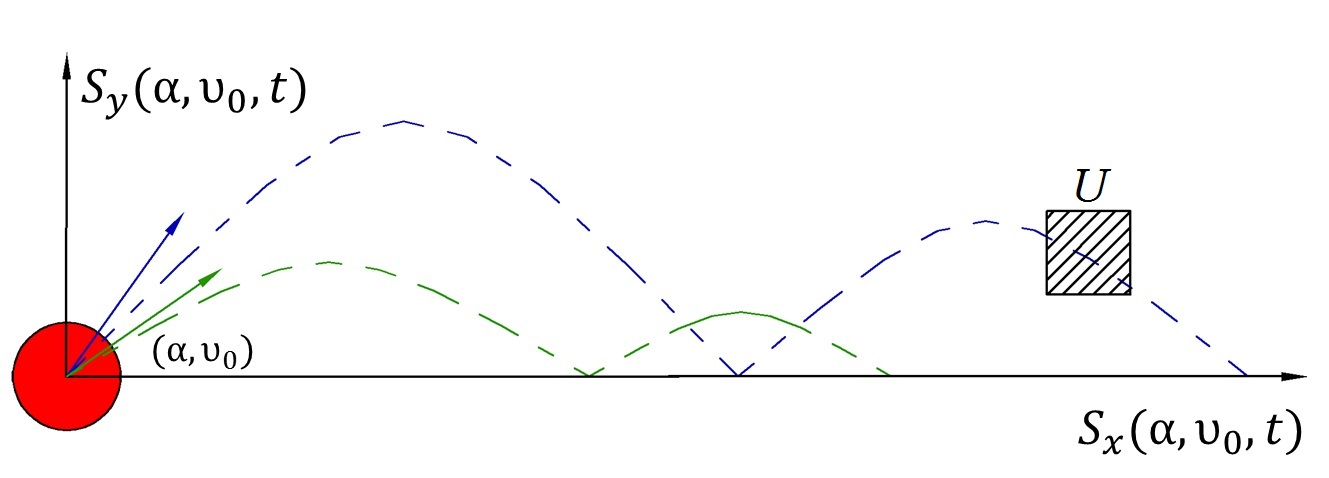
\includegraphics[width=90mm]{bouncing-ball.jpg}
\caption{Bouncing ball scenario}
\end{figure}

The ball trajectory is defined by the system of equations:
\begin{equation} \label{eq:Sx}
S_x(t) = S_{x_0} + \upsilon_0 t \cos{\alpha}
\end{equation}
\begin{equation} \label{eq:Sy}
S_y(t) = S_{y_0} + \upsilon_0 t \sin{\alpha} - \frac{g t^2}{2}
\end{equation}
where $S_x$ and $S_y$ are projections (on the axes $x$ and $y$ respectively) of the distance traveled by the ball starting at the point $(S_{x_0}; S_{y_0})$, $\upsilon_0$ is the initial speed, $\alpha$ is the angle to the horizon, $g$ is a standard gravity and $t$ is time. In this example we assume that the initial point of the ball's center is $(S_{x_0} = 0; S_{y_0} = 0)$

A hybrid system characterizing the behavior of the ball will consists of a single mode with the dynamics defined in (\ref{eq:Sx}) and (\ref{eq:Sy}) and the only jump to the same mode, during which the time $t$ is reset to $0$, the value of $S_x(t)$ before the jump is assigned to the initial value of $S_x(t)$ in the mode after the jump and the speed of the ball is reduced by the coefficient $0.9$.

In order to comply with the description of the hybrid system with random continuous initial parameters, let $\alpha$ be uniformly distributed over the interval $[0, 0.5]$ with the probability density function $f_{A}(\alpha) = 0.5$. Let $\upsilon_0 = 20$ and $t \in [0, 3]$.

Let us consider a bounded probabilistic reachability problem: \textit{is the probability that 
the system reaches in 4 steps the box $D =  \{Sx \in [90, 91], Sy \in [1, 2]\}$ greater or equal 
to $0.062$}?

The Borel set of continuous parameters is formed as:
\begin{equation*}
\begin{split}
B =\{\alpha: \exists t_{0, q_0}, t_{1, q_0}, t_{2, q_0}, t_{3, q_0} \mathord{\in} [0, T]:\\
(S_{x0} = \upsilon_0 t_{0, q_0} \cos{\alpha}) \\
\wedge (S_{y0} = \upsilon_0 t_{0, q_0} \sin{\alpha} - \frac{gt_{0, q_0}^2}{2}) \wedge 
(S_{y0} = 0) \wedge (t_{0, q_0} > 0) \\
\wedge (S_{x1} = S_{x0} + 0.9 \upsilon_0 t_{1, q_0} \cos{\alpha}) \\
\wedge (S_{y1} = 0.9 \upsilon_0 t_{1, q_0} \sin{\alpha} - \frac{gt_{1, q_0}^2}{2}) \wedge 
(S_{y1} = 0) \wedge (t_{1, q_0} > 0) \\
\wedge (S_{x2} = S_{x1} + 0.9^2 \upsilon_0 t_{2, q_0} \cos{\alpha}) \\
\wedge (S_{y2} = 0.9^2 \upsilon_0 t_{2, q_0} \sin{\alpha} - \frac{gt_{2, q_0}^2}{2})
\wedge (S_{y2} = 0) \wedge (t_{2, q_0} > 0) \\
\wedge (S_{x3} = S_{x2} + 0.9^3 \upsilon_0 t_{3, q_0} \cos{\alpha}) \\
\wedge (S_{y3} = 0.9^3 \upsilon_0 t_{3, q_0} \sin{\alpha} - \frac{gt_{3, q_0}^2}{2}) \wedge \\
(S_{x3} \in [90, 91]) \wedge (S_{y3} \in [1, 2])\}
\end{split}
\end{equation*}

Functions $S_x(\alpha, t)$ and $S_y(\alpha, t)$ are invertible with respect to $\alpha$ on 
the domain $[0, 0.5]\times[0, 3]$. Then by applying Proposition \ref{prop:ivp} the formulated 
reachability problem can be encoded as a SMT formula and solved using dReal:
\begin{multline*} 
\exists \alpha \in B = [\alpha_{min}, \alpha_{max}]:\\
(F_A'(\alpha) = f_A(\alpha)) \wedge (F_A(\alpha_{min}) = 0) \wedge (F_A(\alpha) \ge 0.062) .
\end{multline*}
The actual dReal output on the formula above was as follows:
\begin{verbatim}
SAT with the following box:
 time_0:[0.03127620501613272,
                         0.03127624003371717]
 Fa_t:[0.0625524053632542,
                         0.06255247702735234]
 Fa_0:0
 a_0:[0.4292134593911809, 0.4292134922320248]
 t_10:[1.528734841443786, 1.528734859618606]
 t_20:[1.37586135729942, 1.375861377493665]
 t_30:[1.042516533544058, 1.042516555982107]
 t_0:[1.813824229846001, 1.813824261219404]
 t_1:[1.632441880862484, 1.63244191572182]
 t_2:[1.46919748799121, 1.469197526723806]
 t_3:[0.8312598060237518, 0.8312598490599685]
 t_00:[1.698594379660991, 1.698594396018329]
 a_t:[0.4604896994248981, 0.460489732265742]
\end{verbatim}

The probability of reaching the unsafe region by the system thus falls into the interval 
$[0.0625524053632542, 0.06255247702735234]$, that is, the interval associated to the final 
value of $F_A$ (corresponding to \verb#Fa_t# in the printout above). The obtained result was 
validated using a simple Monte Carlo method in MATLAB. The time variable was discretised over 
the interval $[0, 3]$ and the system was simulated using 10,000 uniformly random samples from 
the interval $[0, 0.5]$. The number of samples hitting the unsafe region was 620, thereby 
giving a {\em probabilistic} estimate of $\frac{620}{10,000}= 0.062$. In comparison, our method 
gives an interval of size $0.72\times 10^{-7}$ which is {\em guaranteed} to contain the actual 
probability.




\section{Probabilistic Reachability}
%\begin{equation}
%\int_{\Omega} I_{B}(r)dP(r)
%\end{equation}
%where $dP(r)$ is a probability measure of the random variable and $Id_{B}$ is the indicator function defined as:
%\begin{equation}
%	I_{B}(r) = 
%	\begin{cases}
%		1, \text{if the system reaches $U$ on $k$-th step} \\
% 		0, \text{otherwise}
%	\end{cases}
%\end{equation}
We now present a more general procedure for calculating the probability of reaching 
the unsafe region in $k$ steps. The procedure works for general hybrid systems
whose dynamics is given implicitly, \eg, as a solution of ODEs. In particular, we do not
require the dynamics to be invertible with respect to the random parameter. The main idea 
is to compute the probability by integrating an indicator function over the probability measure 
of the random variable as:
\begin{equation*}
\int_{\Omega} I_{U}(r)dP(r)
\end{equation*}
where $P(r)$ is a probability measure of the random variable, $\Omega$ is the range of the 
random variable, and $I_{U}$ is the indicator function defined as:
\begin{equation*}
        I_{U}(r) = 
        \begin{cases}
                1, \text{system with parameter $r$ reaches $U$ in $k$-steps} \\
                0, \text{otherwise}
        \end{cases}
\end{equation*}
The procedure for solving probabilistic reachability thus consists of a validated integration 
procedure and a $\delta$-complete decision procedure used for verifying the indicator function
(and thus building the set $B$).

\noindent{\em Notation.}
For an interval $[r]=[\underline{r}, \overline{r}] \subset \mathbb{R}$ we denote the size of
the interval by $width([r]) = \overline{r} - \underline{r}$ and by                         
$mid([r]) = \frac{\overline{r} + \underline{r}}{2}$ the central point of the interval.

\subsection{Validated Integration Procedure}
In the implementation of a validated integration procedure we employ the (1/3) Simpson rule:
\begin{equation}\label{eq:Simpson}
\begin{split}
K= \int_{a}^{b} \, f(x)\, dx\, = \frac{width([I])}{6}(f(a) + \\
4 f(mid([I])) + f(b)) - \frac{width([I])^5}{2880}f^{(4)}(\xi)
\end{split}
\end{equation}
where $I=[a,b]$, $\xi \in [I]$ and $f^{(4)}$ is the fourth derivative of $f$.
Applying interval arithmetics an interval extension of function $f$ and its fourth derivative 
can be obtained.
\begin{definition}
An interval extension of a function $f:X \rightarrow Y$ is an operator $[\cdot]$ such that:
\begin{equation*}
	\forall x \in [r] \subseteq X: f(x) \in [f]([r]) \subseteq Y
\end{equation*}
\end{definition} 

The interval version of Simpson's rule can be obtained simply by replacing in (\ref{eq:Simpson})
occurences of $f$ and $f^{(4)}$ with their interval extension $[f]$, and by replacing $\xi$ with
the entire $[a,b]$ interval \cite{ValidatedIntegration}:
\[
\begin{split}
K \in [K]([a, b]) = \frac{width([I])}{6}([f](a) + 4 [f](mid([I])) + \\
[f](b)) - \frac{width([I])^5}{2880}[f]^{(4)}([I]).
\end{split}
\]
Furthermore, by definition of integral:
\[
\begin{split}
K \in \Sigma_{i = 1}^{n} [K]([x]_{i})
\end{split}
\]
where $n$ is a number of disjoint intervals $[x]_{i}$ in $[a, b]$. Interval extensions can
be readily computed using interval arithmetics libraries such as FILIB++ \cite{filib}.

In order to guarantee $\delta$-completeness of the integration it is sufficient to divide 
$[a, b]$ into $n$ disjoint intervals $[x]_{i}$ such that for each $[x]_{i}$ we have
$width([I]([x]_{i})) < \delta \frac{width([x]_{i})}{b - a}$. Then the exact value of the 
integral will be within an interval of width smaller than $\delta$. Pseudo-code for the 
procedure computing the integral up to an arbitrary $\delta \in \mathbb{Q}^{+}$ is given 
in Algorithm \ref{alg:integration}.

\begin{algorithm}
\label{alg:integration}
input: $f(x)$, $[a, b]$, $\delta$\;
output: $[I]$\;
$B$.push($[a, b]$)\;
$[I] = [0.0, 0.0]$\;
\While{$size(B) > 0$}{
	$[x]$ = $B$.pop()\;
	$[S]([x]) = \frac{width([x])}{6}([f](\underline{x}) + 4 [f](mid([x])) + [f](\overline{x})) - \frac{(width([x]))^5}{2880}[f^{(4)}]([x])$\;
	\If{$width([S]([x])) > \delta \frac{width([x])}{b - a}$}{
		$B$.push($[\underline{x}, mid([x])]$)\;
		$B$.push($[mid([x]), \overline{x}]$)\;
	}\Else{
		$[I] = [I] + [S]([x])$\;
	}
}
\Return $[I]$\;
\caption{Validated Integration Procedure}
\end{algorithm}

\subsection{Borel set}
Now we need to correctly identify the Borel set, or equivalently, verifying the indicator function
above. Let $\phi$ be a formula of the form:
\begin{equation} \label{eq:phi}
\begin{split}
\phi([r]) = \exists \rho \in [r], \exists \textbf{x}^{0}_{0,q_0}, \exists \textbf{x}^{t}_{0,q_0}, \exists t_{0, q_0}, ... , \exists \textbf{x}^{0}_{0,q_m}, \\ \exists \textbf{x}^{t}_{0,q_m}, \exists t_{0, q_m}, ... , \exists \textbf{x}^{0}_{k,q_m}, \exists \textbf{x}^t_{k,q_m}, \exists t_{k, q_m}:\\
(\bigvee_{q \in Q} (\text{init}_{q}(r, \textbf{x}^{0}_{0,q}) \wedge \text{flow}_{q}(r, \textbf{x}^{0}_{0,q}, \textbf{x}^{t}_{0,q}))) \wedge \\
(\bigwedge_{i=0}^{k-1} (\bigvee_{q,q' \in Q}(\text{jump}_{q \rightarrow q'}(r, \textbf{x}^{t}_{i,q}, \textbf{x}^{0}_{i+1,q'}) \wedge \\
(\text{flow}_{q'}(r, \textbf{x}^{0}_{i+1,q'}, \textbf{x}^{t}_{i+1,q'}))) \wedge (\bigvee_{q \in Q} \text{unsafe}_{q}(r, \textbf{x}^{t}_{k,q}))))
\end{split}
\end{equation}
If the formula is true then $[r]$ contains a value such that the system initial random parameter 
reaches the unsafe region.

Taking a complement of the unsafe region $U^{C} = S / U$ (where $S$ is the state space of the 
system) and defining a predicate $\text{unsafe}^{C}_{q}(r,\textbf{x}^{t})$ evaluating to true iff
$s = (q, r, \textbf{x}^{t}_{q}) \in U^{C}$ we want to ensure that the system never reaches the 
unsafe region {\em within} the $k$-th step with an initial random parameter from $[r]$. 
In order to conclude that it is sufficient to evaluate the formula:
\begin{equation} \label{eq:phi_C}
\begin{split}
\phi^{C}([r]) = 
	\exists \rho \in [r], \exists \textbf{x}^{0}_{0,q_0}, \exists \textbf{x}^{t}_{0,q_0}, \exists t_{0, q_0} , ... , \exists \textbf{x}^{0}_{0,q_m}, \\
\exists \textbf{x}^{t}_{0,q_m}, \exists t_{0, q_m}, ... , \exists \textbf{x}^{0}_{k,q_m}, \exists \textbf{x}^t_{k,q_m}, \exists t_{k, q_m}, \forall t'_{k, q_m} \in [0, t_{k, q_m}]:\\
(\bigvee_{q \in Q} (\text{init}_{q}(r, \textbf{x}^{0}_{0,q}) \wedge \text{flow}_{q}(r, \textbf{x}^{0}_{0,q}, \textbf{x}^{t}_{0,q}))) \wedge \\
(\bigwedge_{i=0}^{k-1} (\bigvee_{q,q' \in Q}(\text{jump}_{q \rightarrow q'}(r, \textbf{x}^{t}_{i,q}, \textbf{x}^{0}_{i+1,q'}) 
\wedge \\
(\text{flow}_{q'}(r, \textbf{x}^{0}_{i+1,q'}, \textbf{x}^{t}_{i+1,q'}))) \wedge \\
(\bigvee_{q \in Q} (\text{unsafe}^{C}_{q}(r, \textbf{x}^{t}_{k,q}) \wedge (\text{jump}_{q \rightarrow q'}(r, \textbf{x}^{t}_{k,q}, \textbf{x}^{0}_{k+1,q'})))))
\end{split}
\end{equation}
If the formula evaluates to true then the system does not reach the unsafe region on the $k$-th step.
Then set $B$ can be defined as the collection
$\{[r]_{i} : \phi([r]_{i}) \wedge (\neg \phi^{C}([r]_{i})\}$.

\subsection{Probabilistic reachability}
Integrating a probability density function of a random variable we obtain intervals 
such that size of the enclosure containing the exact value of a partial sum for each 
of them is smaller than a local error.

Then a decision about the relation between each of the obtained intervals and the (unknown) 
Borel set $B$ should be taken. In order to achieve this we use a $\delta$-complete decision 
procedure, \ie, dReal, to verify formulas (\ref{eq:phi}) and (\ref{eq:phi_C}). The following 
three outcomes are considered:
\begin{itemize}
	\item{$\phi([r])$ is $\delta$-\textbf{sat} and $\phi^C([r])$ is \textbf{unsat}}
	\item{$\phi([r])$ is \textbf{unsat}}
	\item{$\phi([r])$ is $\delta$-\textbf{sat} and $\phi^C([r])$ is $\delta$-\textbf{sat}}
\end{itemize}

In the first case, we can conclude that $[r] \cap B = [r]$. Therefore, $[r] \subseteq B$ and 
the value of the partial sum on this interval should be added to the resulting value of the 
integral. The second case allows concluding that $[r] \cap B = \emptyset$. Hence, this interval 
can be completely removed from the integration domain. Finally, in the last case, 
$[r] \cap B \ne \emptyset$ and $[r] \cap B \ne [r]$. In other words, the interval $[r]$ is not 
fully contained in the set $B$. Hence, this interval should be split into two subintervals and 
each of them should be checked in the same way.

After each run through the set of intervals $[r]_{i}$, the over-approximated $[I_{over}]$ and 
under-approximated $[I_{under}]$ interval values of the integral are calculated. The 
under-approximated value is calculated only over the intervals fully contained in set $B$ 
while the over-approximation of the integral involves values of partial sum on the intervals 
which are either fully or partially contained in set $B$. The exact value of the integral will 
always be within the interval $[\underline{I_{under}}, \overline{I_{over}}]$. The algorithm 
terminates when the length of the interval $[\underline{I_{under}}, \overline{I_{over}}]$ is 
smaller than $\delta$. Pseudo-code for the procedure is presented in Algorithm \ref{alg:prob-reach}.
\begin{algorithm}
\label{alg:prob-reach}
input: $f(x)$, $[a, b]$, $\delta_{1}$, $\delta_{2}$, $\phi$, $\phi^C$\;
output: $[I]$\;
\tcp{stack for all the intervals}
$B$.push($[a, b]$)\;
\tcp{stack only for the intervals and partial sum satisfying a local error}
$T = \emptyset$\;
\While{$size(B) > 0$}
{
	$[x]$ = $B$.pop()\;
	$[S]([x]) = \frac{width([x])}{6}([f](\underline{x}) + 4 [f](mid([x])) + [f](\overline{x})) - \frac{(width([x]))^5}{2880}[f^{(4)}]([x])$\;
	\If{$width([S]([x])) > \delta_{1} \frac{width([x])}{b - a}$}
	{
		$B$.push($[\underline{x}, mid([x])]$)\;
		$B$.push($[mid([x]), \overline{x}]$)\;
	}\Else
	{
		$T$.push($\{[x], [S]([x])\}$)\;
	}
}

$[I_{under}] = [0.0, 0.0]$\;
$[I_{over}] = [0.0, 0.0]$\;
$[I] = [0.0, 1.0]$\;
\tcp{stack containing extra divisions of the intervals}
$D = \emptyset$\;
\While{$width([I]) > \delta_{2}$}
{
	\While{$size(T) > 0$}
	{
	$\{[x], [S]([x])\} = T$.pop()\;
	\If{$\phi([x])$}
	{
		$[I_{over}] = [I_{over}] + [S]([x])$\;
		\If{$\phi^{C}([x])$}
		{
			$D$.push($\{[\underline{x}, mid([x])], [S([\underline{x}, mid([x])])]\}$)\;
			$D$.push($\{[mid([x])], \overline{x}, [S([mid([x])], \overline{x})]\}$)\;
		}\Else
		{
			$[I_{under}] = [I_{under}] + [S]([x])$\;
		}
	}
	$[I] = [\underline{I_{under}}, \overline{I_{over}}]$\;
	$[I_{over}] = [I_{under}]$\;
	$T = D$\;
	$D = \emptyset$\;	
	}
}

\Return $[I]$\;

\caption{Probabilistic $\delta$-reachability}
\end{algorithm}


\section{Case Study}
% PZ: I think the two sentences below should in 'Methods' section.
%We have developed an open-source tool dReach using OCaml to perform $\delta$-complete reachability 
%analysis for hybrid systems \cite{dreach}. dReach is built upon our SMT solver dReal \citep{dreal} 
%that implements a $\delta$-complete decision procedure. 

To exemplify different aspects of our parameter synthesis framework, we carried out a case study on
a model of the electrical dynamics of cardiac cells. All the experiments reported below were done 
using a machine with two Intel Xeon E5-2650 2.00GHz processors and 64GB RAM. The precision $\delta$
was set to $0.001$.

\begin{figure}[t]
\centering
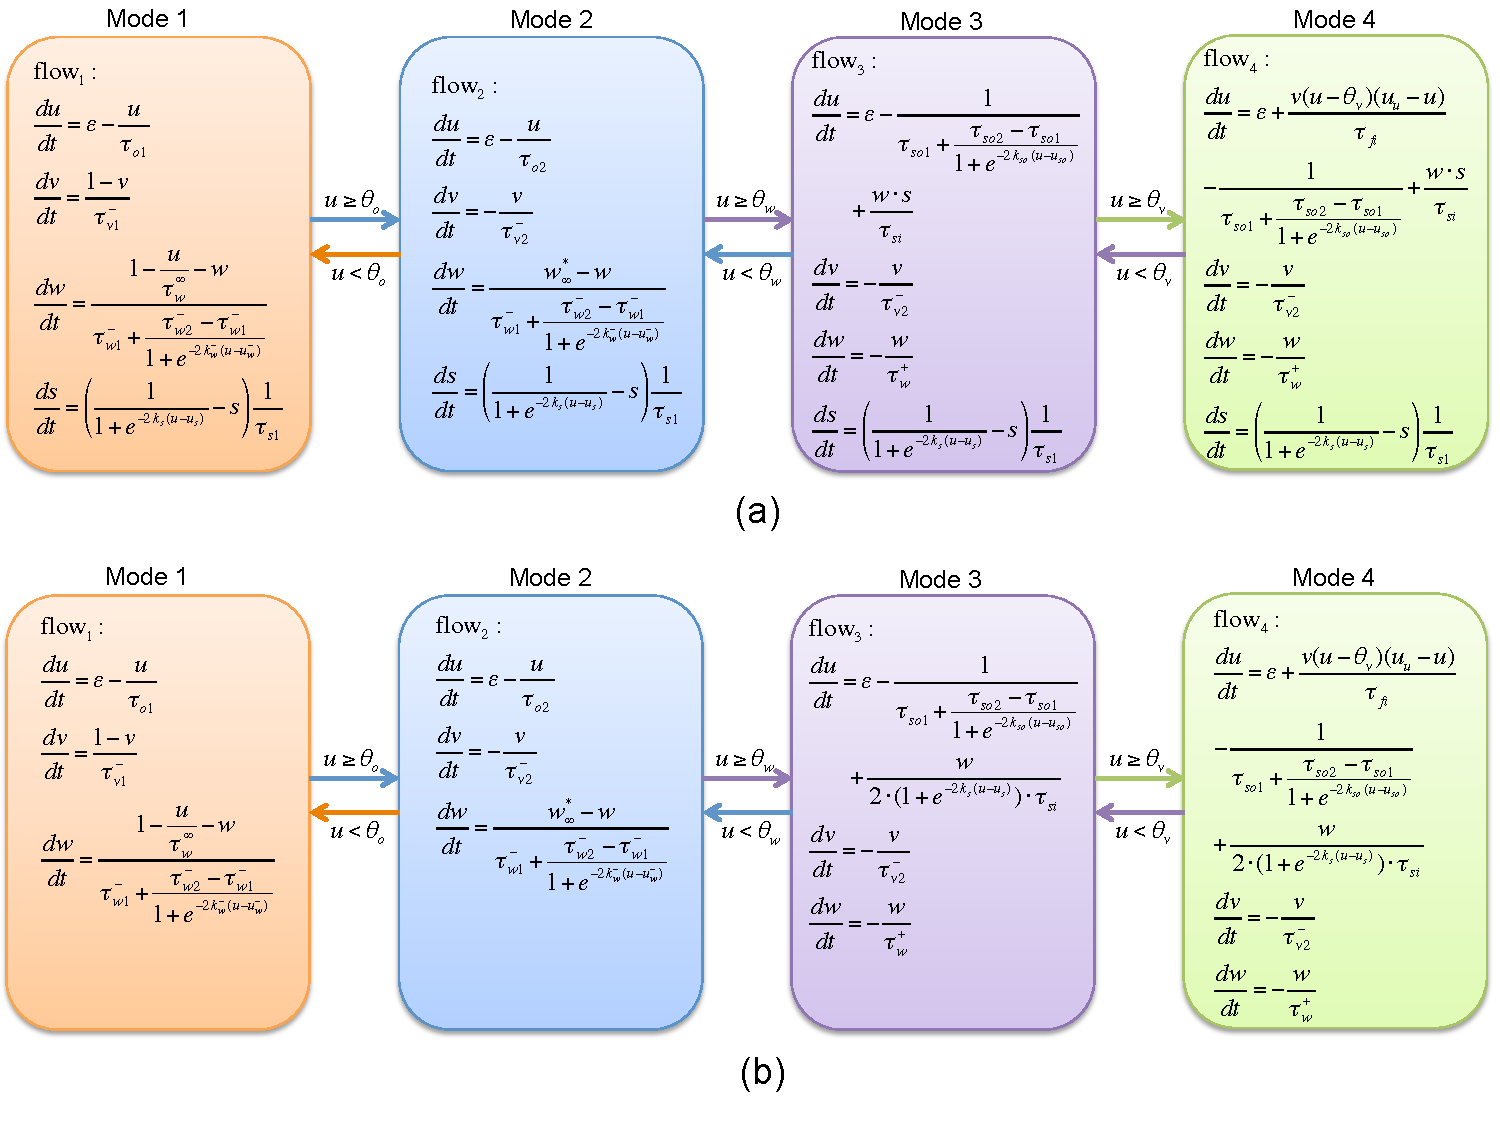
\includegraphics[scale=0.5]{fig-cardiac-new}
\caption{Hybrid models of cardiac cells. (a) BCF model. (b) FK model.}
\label{model}
 %\vspace{-0.7cm}
\end{figure}

\subsection{Hybrid models of cardiac cells}
The heart rhythm is enabled by the electrical activity of cardiac muscle cells, which make up the atria and ventricles. The electrical dynamics of cardiac cells is governed by the organized opening and closing of ion channel gates on the cell membrane. Improper functioning of the cardiac cell ionic channels can cause the cells to lose excitability, which disorders electric wave propagation and leads to cardiac abnormalities such as ventricular \textit{tachycardia} or \textit{fibrillation}. Hybrid automata models have been developed recently in order to understand the mechanisms of cardiac disorders, including the Fenton-Karma (FK) model \cite{fenton98} and the Bueno-Cherry-Fenton (BCF) model \cite{orovio08}. 

\paragraph{BCF Model.} 
In this model, the change of cells transmembrane potential $u$, in response to an external stimulus $\epsilon$ from neighboring cells, is regulated by a fast ion channel gate $v$ and two slow gates $w$ and $s$.
Figure \ref{model}(a) shows the four modes associated with the BCF model. In Mode $1$, gates $v$ and $w$ are open and gate $s$ is closed. The transmembrane potassium current causes the decay of $u$. The cell is resting and waiting for stimulation. We assume an external stimulus $\epsilon$ equals to $1$ which lasts for $1$ millisecond. The stimulation causes $u$ to increase, which may trigger $\jump_{1 \rightarrow 2}: u \geq \theta_o$. When this jump takes place, the system switches to Mode 2 and $v$ starts closing, and the decay rate of $u$ changes. The system will jump to Mode 3 if $u \geq \theta_w$. In Mode 3, $w$ is also closing; $u$ is governed by the potassium current and the calcium current. When $u \geq \theta_v$, Mode 4 can be reached, which signals a successful action potential (AP) initiation. In Mode 4, $u$ reaches its peak due to the fast opening of the sodium channel. The cardiac muscle contracts and $u$ starts decreasing. 

\paragraph{FK Model.} 
As shown in Figure \ref{model}(b), this model comprises the same four modes and equations of the BCF model, except that the current change induced by gate $s$ is reduced to an explicit term which is integrated
in the right-hand side of $du/dt$. Similarly to the BCF model, an AP can be successfully initiated when Mode 4 is reached. 

We specified both the BCF and the FK model using dReach's modeling language. Starting from the state ($u = 0$, $v = 1$, $w = 1$, $s = 0$) in Mode 1, we checked whether Mode 4 is reachable using the parameter values presented in \cite{orovio08}. This was true (\ie, dReach returned $\delta$-$\mathsf{sat}$) for both models. 
The simulation of a few witness trajectories are shown in Figure \ref{trace} (the stimulus $\epsilon$ was reset every $500$ milliseconds).


\begin{figure}[thb]
\centering
\subfigure[]{
  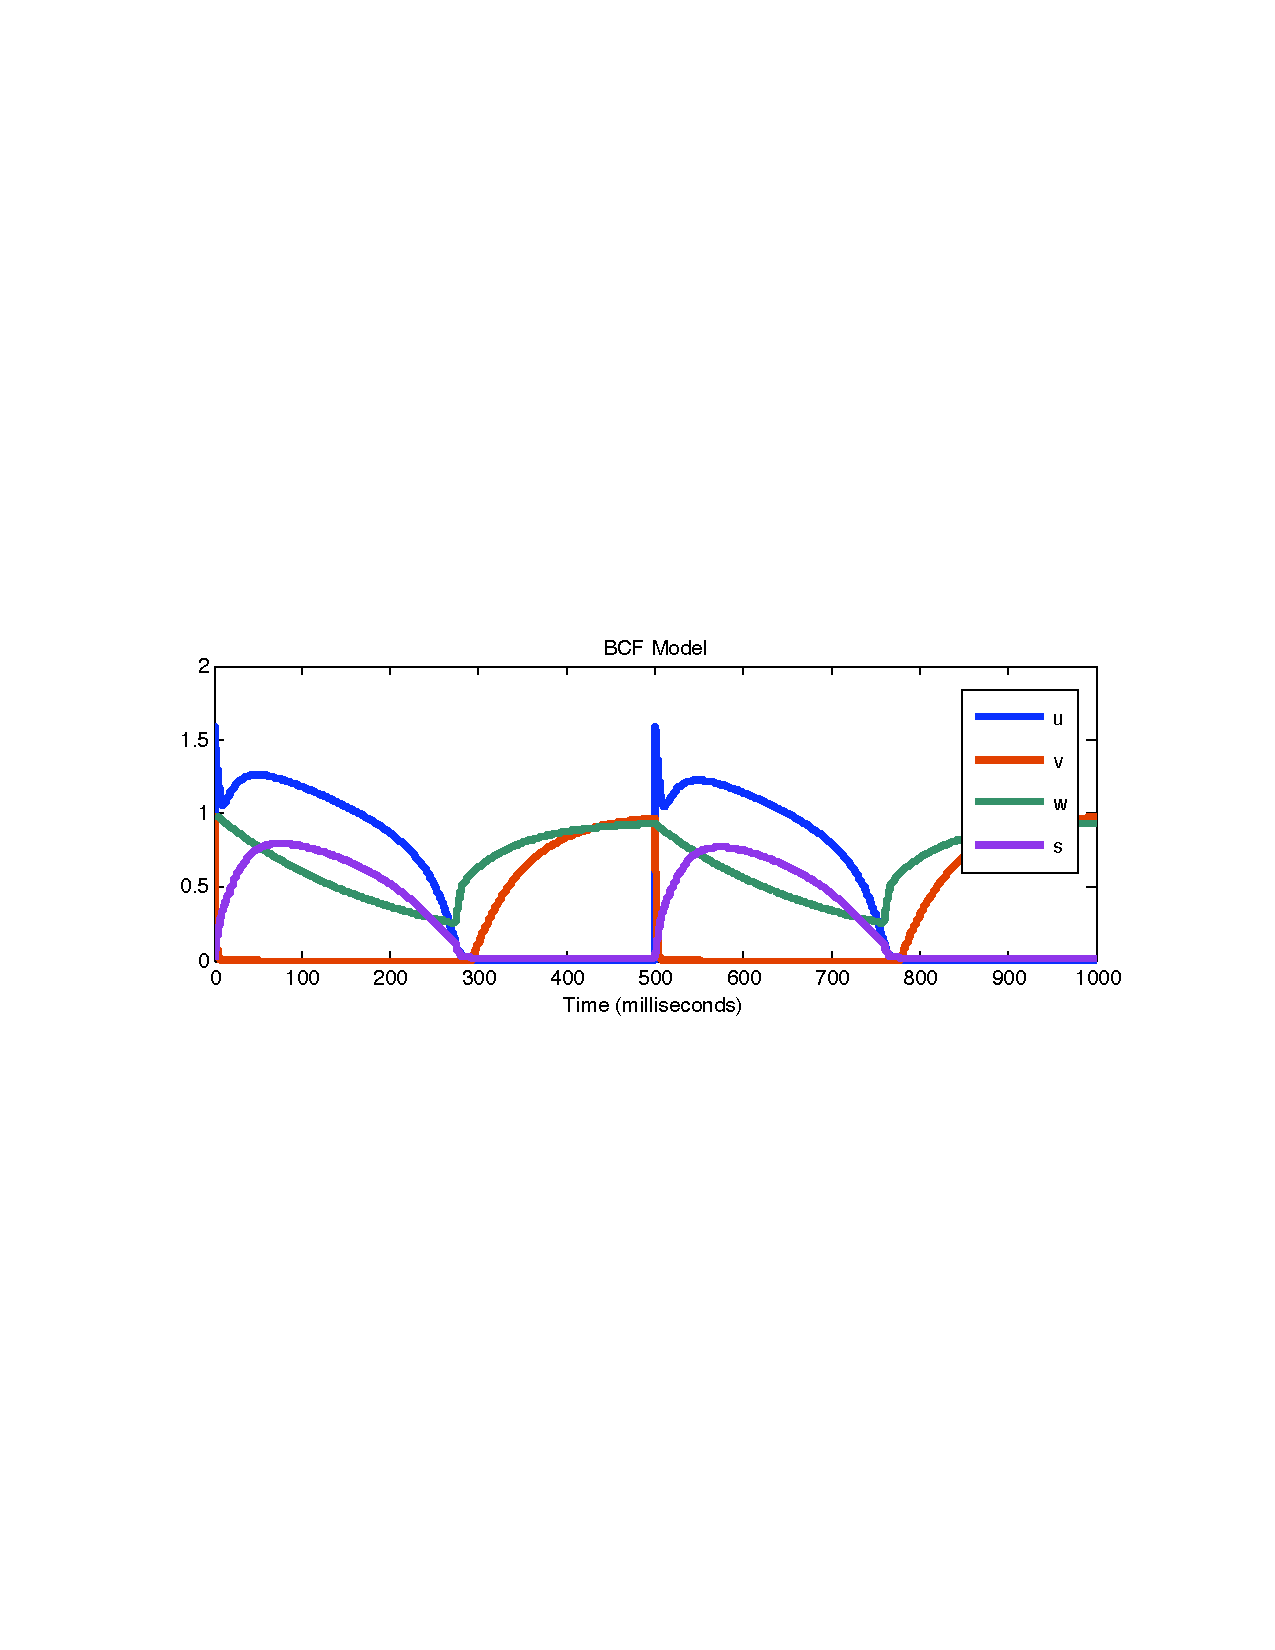
\includegraphics[width=8cm]{fig-bcf}
} 
\subfigure[]{
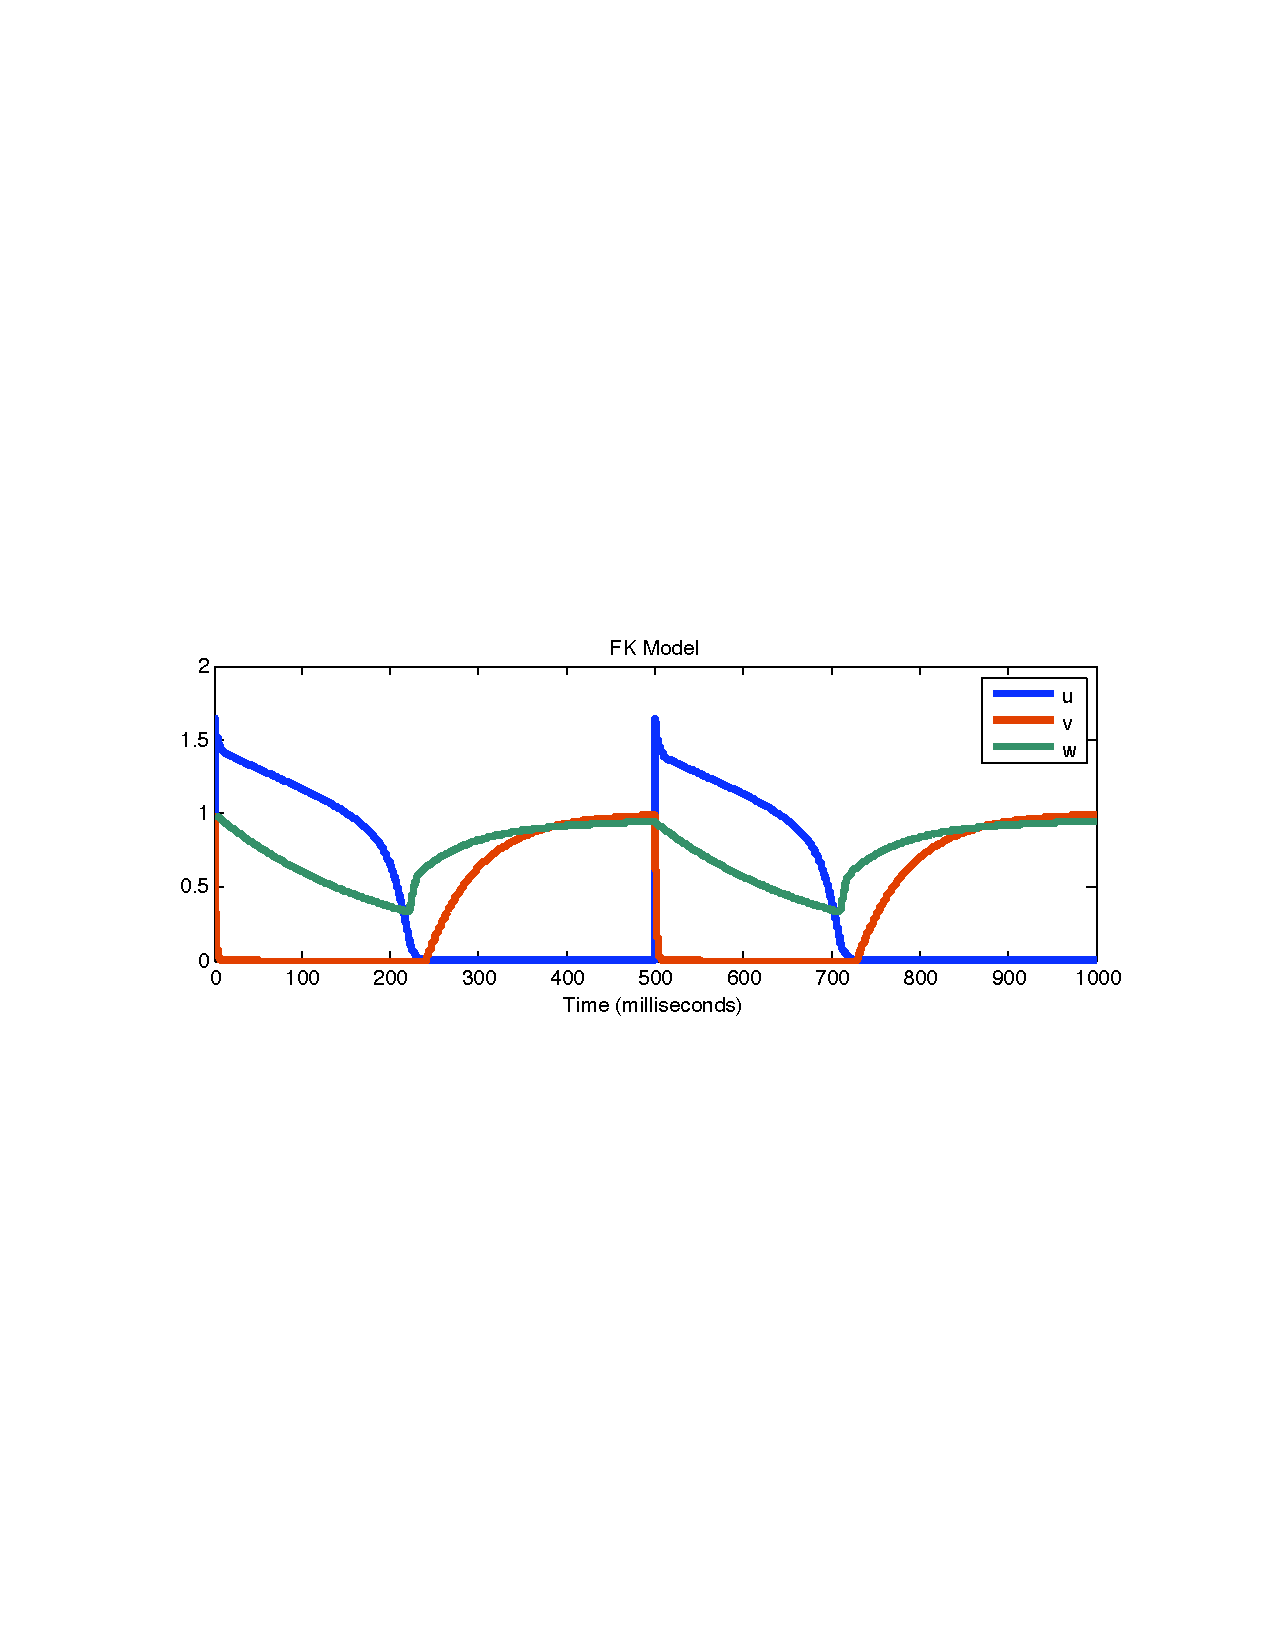
\includegraphics[width=8cm]{fig-fk}
}
\caption{The simulated time profile of BCF and FK.}
\label{trace}
 %\vspace{-0.7cm}
\end{figure}


\subsection{Model falsification}
Both the BCF and FK models were able to reproduce essential characteristics (\eg, steady-state action potential duration) observed in human ventricular cells \cite{fenton98,orovio08}. However, ventricular cells comprise three cell types, which possess different dynamical characteristics. For instance, Figure \ref{ap} shows that time courses of APs for epicardial and endocardial human ventricular cells have different morphologies \cite{nabauer96}. An important \textit{spike-and-dome} AP morphology can only be observed in epicardial cells but not endocardial cells. Hence, in a model-based study, one needs to identify cell-type-specific parameters to take account into cellular heterogeneity. The feasibility of this task will depend on the model of choice, as certain model would be impossible to reproduce a dynamical behavior no matter which parameter values are used. Here we illustrate that such models can be ruled out efficiently using our $\delta$-decision based parameter synthesis framework.

\paragraph{Robustness.} 
To ensure proper functioning of cardiac cells in noisy environments, an important property of the system is to filter out insignificant stimulation. Thus, we expected to see that APs could not be initiated for small $\epsilon$. Starting from the state ($u = 0$, $v = 1$, $w = 1$, $s = 0$, $\epsilon \in [0.0,0.25]$) in Mode 1, we checked the reachability of Mode 4. The $\mathsf{unsat}$ answer was returned by dReach for both the BCF and FK
model, showing that the models are robust to stimulation amplitude.

\begin{figure}[th]
\centering
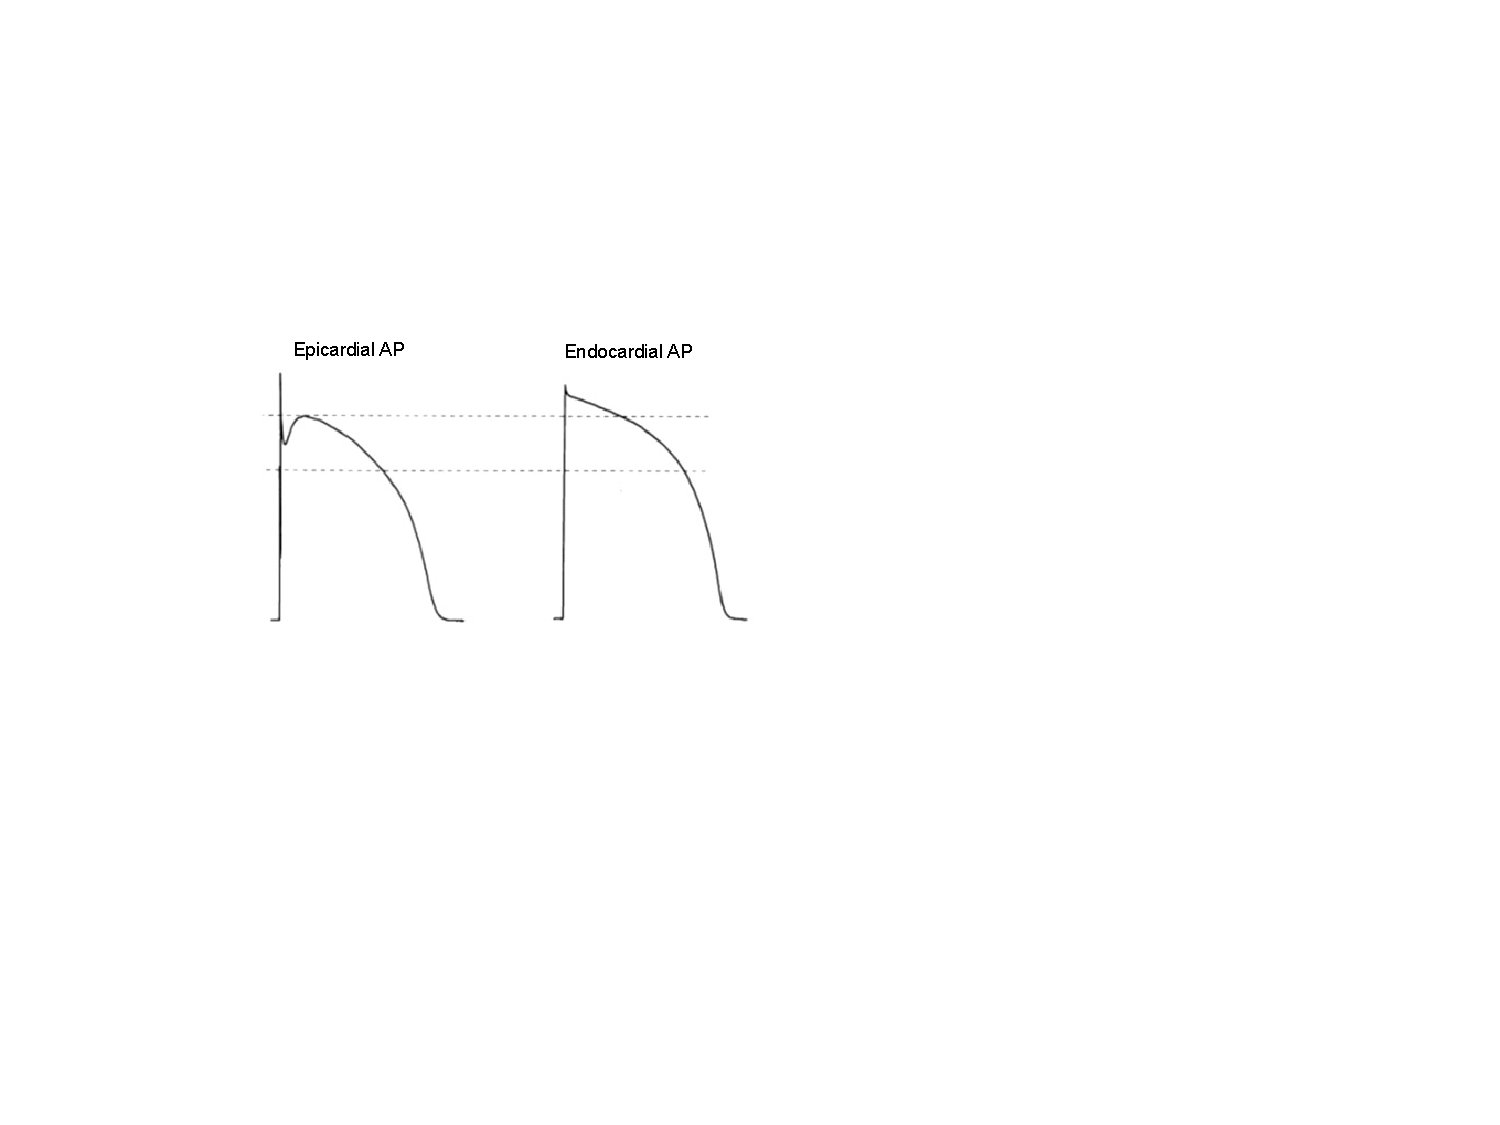
\includegraphics[scale=0.8]{fig-ap}
\caption{Experimental AP morphology \cite{nabauer96}.}
\label{ap}
 %\vspace{-0.7cm}
\end{figure}

\paragraph{AP morphology.}
Next we tested whether the models can reproduce the spike-and-dome AP morphology of epicardial cells. We introduced two auxiliary modes (Mode 5 and 6). The system will jump from Mode 4 to Mode 5 if $\tau \le 10$, and will jump from Mode 5 to Mode 6 if $\tau \le 30$. In Modes 5 and 6, we enforced invariants $1.0 \le u \le 1.15$ and $1.18 \le u \le 2.0$, respectively, to depict the spike-and-dome morphology observed experimentally \cite{nabauer96}. We then checked reachability of Mode 6, starting from Mode 1 in state ($u = 0$, $v = 1$, $w = 1$, $s = 0$, $\epsilon \in [0.9,1.1]$, $\tau_{si} \in [1,2]$, $u_s \in [0.5,2]$). The $\delta$-$\mathsf{sat}$ answer
was returned for BCF, while $\mathsf{unsat}$ was returned for FK, indicating that the FK model cannot reproduce spike-and-dome shapes using reasonable parameter values. Hence, FK is not suitable to study the dynamics of epicardial cells.

We remark that any $\mathsf{unsat}$ answer is guaranteed to be correct. This effectively
means that we proved that the FK model cannot reach Mode 6 for {\em any} starting state in the 
rectangle ($u = 0$, $v = 1$, $w = 1$, $s = 0$, $\epsilon \in [0.9,1.1]$, $\tau_{si} \in [1,2]$, 
$u_s \in [0.5,2]$). Sampling-based approaches cannot have the same level of certainty, while other
approaches cannot handle the complexity of the flows in the model.


\subsection{Parameter identification for cardiac disorders}

When the system cannot reach Mode 4, the cardiac cell loses excitability, which might lead to tachycardia or fibrillation. Starting with Mode 1, our next goal was to identify parameter ranges for which the system will never go into Mode 4. In what follows, we focused our study on the BCF model. 
Grosu {\em et al.}~\cite{grosu11} have tackled this parameter identification problem by linearizing the BCF model into a piecewise-multiaffine system (referred as MHA). With this simplification, parameter ranges could be identified using the Rovergene tool \cite{rovergene}. However, the BCF and MHA models have different sets of parameters. Here we aimed at identifying disease-related ranges of the original BCF parameters. It can be derived from the model equations that $\tau_{o1}$ and $\tau_{o2}$ govern the dynamics of $u$ in Mode 1 and Mode 2 respectively, and hence determine whether $\jump_{1\rightarrow 2}$ and  $\jump_{2\rightarrow 3}$ can be triggered. For $\tau_{o1}$, we performed a binary search in value domain $[0.0001,0.01]$ to obtain a threshold value $\theta_{o1}$ such that Mode 4 is unreachable if $\tau_{o1} \in (0, \theta_{o1})$ while Mode 4 is reachable if $\tau_{o1} =  \theta_{to1}$. Specifically, for each candidate value $\theta^i_{o1}$, we checked the reachability of Mode 4 with the initial state ($u = 0$, $v = 1$, $w = 1$, $s = 0$, $\theta_{o1} = \theta^i_{o1}$). We set the next candidate to be $(\theta^i_{o1} -\theta_{l})/2$ if $\mathsf{sat}$ was returned, or $(\theta_{r} - \theta^i_{o1})/2$ if $\mathsf{unsat}$ was returned, where $\theta_{l}$ is the largest $\mathsf{unsat}$ candidate and $\theta_{r}$ is the smallest $\mathsf{sat}$ candidate. 

In this manner, we identified $\theta_{o1}$ to be $0.006$, which suggest that when $\tau_{o1} \in (0, 0.006)$, the system will always stay in Mode 1. Similarly, we also obtained a threshold value of $0.13$ for $\tau_{o2}$, such that Mode 3 cannot be reached when $\tau_{o2} \in (0, 0.13)$. Furthermore, whether the system can jump from Mode 3 to Mode 4 depends on the interplay between $\tau_{so1}$ and $\tau_{so2}$.  For each value $\tau_{so2}^i$ of $\tau_{so2}$ sampled from domain $(0, 100]$, we performed the binary search in $(0, 5]$ to find the threshold value $\theta_{so1}$ such that Mode 4 is unreachable when $\tau_{so1} \in [0,\theta_{so1}]$ and $\tau_{so2} = {\tau_{so2}^i}$. By linear regression of the obtained values of $\theta_{so1}$, we identified one more condition that Mode 4 is unreachable:  $6.2 \cdot \tau_{so1} + \tau_{so2} \ge 9.9$. Taken together, we identified the following disease-related parameter ranges:  
$$\tau_{o1} \in (0,0.006)\vee \tau_{o2} \in (0,0.13)\vee 6.2 \cdot \tau_{so1} + \tau_{so2} \ge 9.9$$
Figure \ref{cresults} visualizes these results by showing the simulated trajectories using corresponding  parameter values.

I THINK WE NEED:
\begin{itemize}
	\item A TABLE WITH ALL THE RESULTS AND RUNTIMES
	\item PSEUDO-CODE FOR THE BINARY SEARCH ALGO
\end{itemize}


\begin{figure}[h]
\centering
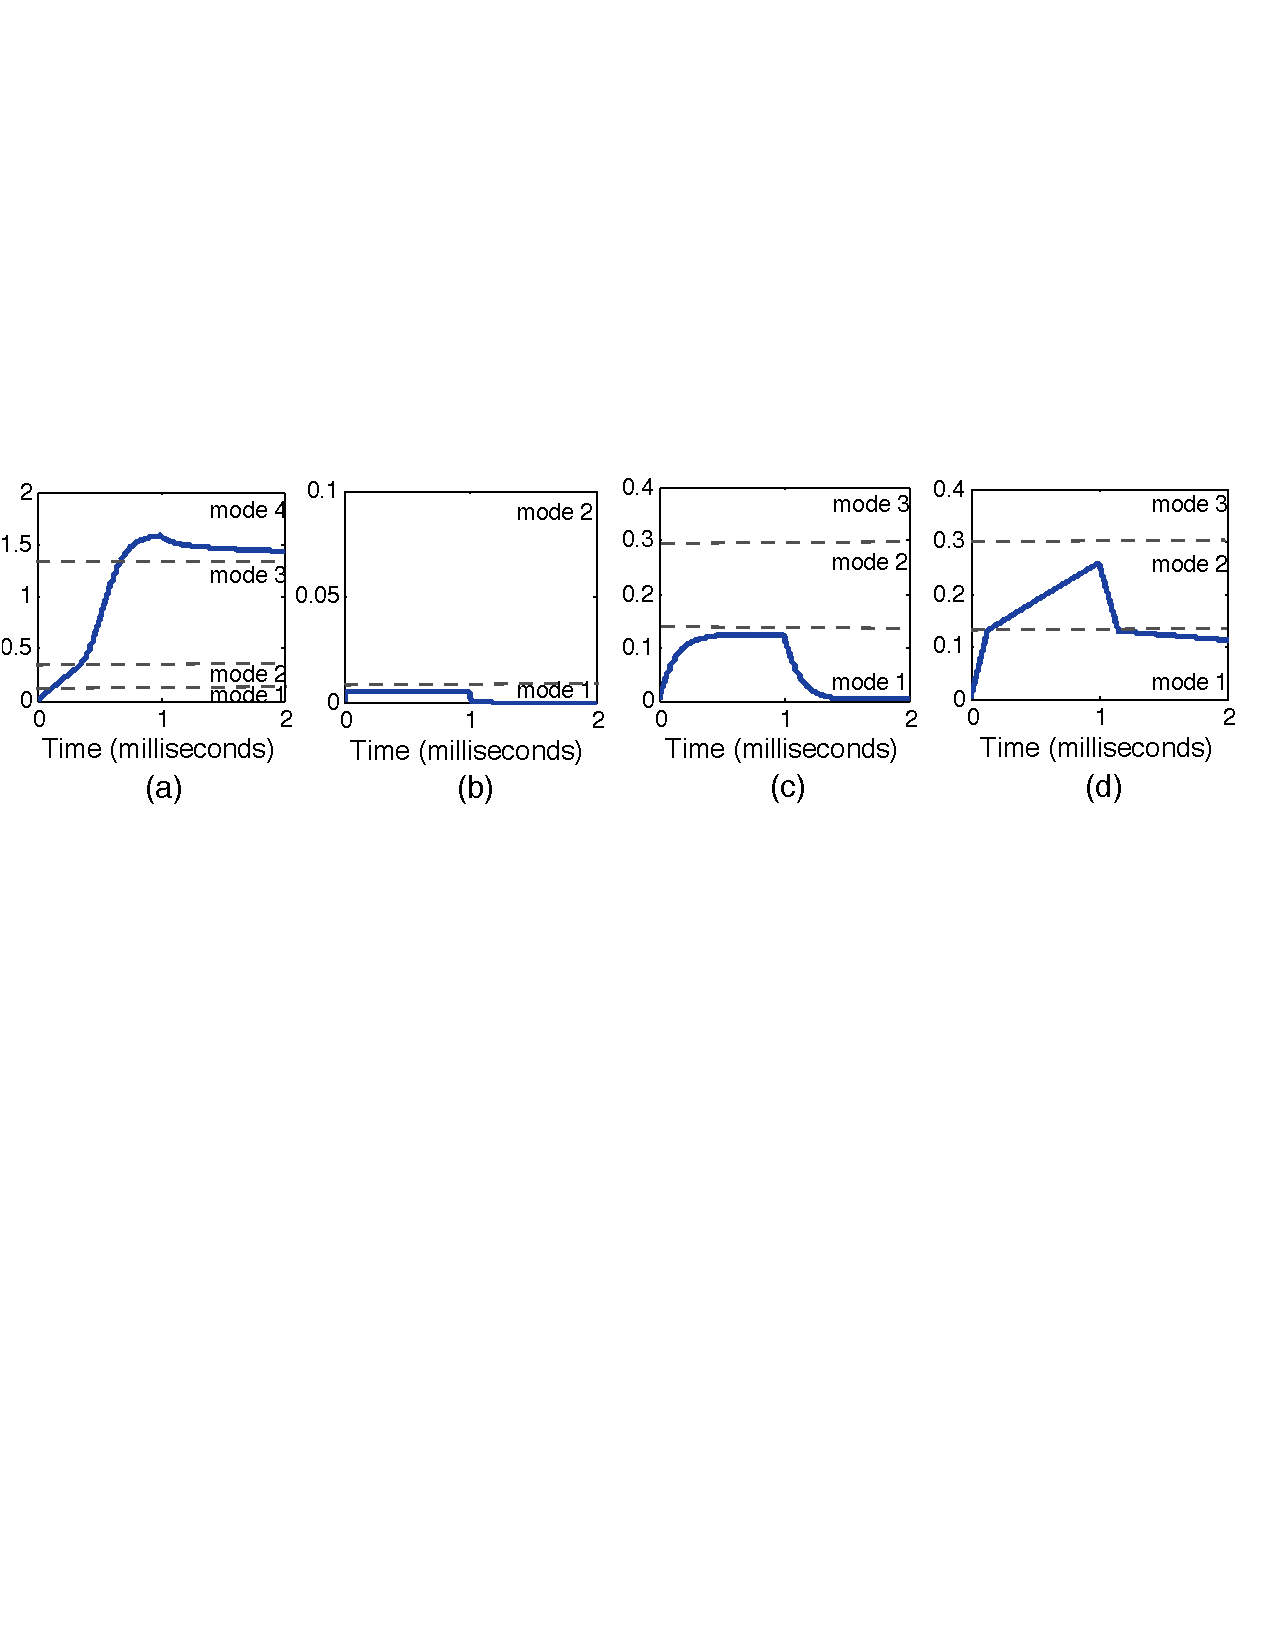
\includegraphics[scale=0.6]{fig-cardiactraj2}
\caption{Simulation results using disease related parameter values. (a) Original parameters (b) $\tau_{o1}=0.0055$ (c) $\tau_{o2} = 0.125$ (d) $\tau_{so1} =1.2$, $\tau_{so2} =1.0$ }
\label{cresults}
 %\vspace{-0.7cm}
\end{figure}

%%% Local Variables:
%%% TeX-master: "main"
%%% End:



% An example of a floating figure using the graphicx package.
% Note that \label must occur AFTER (or within) \caption.
% For figures, \caption should occur after the \includegraphics.
% Note that IEEEtran v1.7 and later has special internal code that
% is designed to preserve the operation of \label within \caption
% even when the captionsoff option is in effect. However, because
% of issues like this, it may be the safest practice to put all your
% \label just after \caption rather than within \caption{}.
%
% Reminder: the "draftcls" or "draftclsnofoot", not "draft", class
% option should be used if it is desired that the figures are to be
% displayed while in draft mode.
%
%\begin{figure}[!t]
%\centering
%\includegraphics[width=2.5in]{myfigure}
% where an .eps filename suffix will be assumed under latex, 
% and a .pdf suffix will be assumed for pdflatex; or what has been declared
% via \DeclareGraphicsExtensions.
%\caption{Simulation Results}
%\label{fig_sim}
%\end{figure}

% Note that IEEE typically puts floats only at the top, even when this
% results in a large percentage of a column being occupied by floats.


% An example of a double column floating figure using two subfigures.
% (The subfig.sty package must be loaded for this to work.)
% The subfigure \label commands are set within each subfloat command, the
% \label for the overall figure must come after \caption.
% \hfil must be used as a separator to get equal spacing.
% The subfigure.sty package works much the same way, except \subfigure is
% used instead of \subfloat.
%
%\begin{figure*}[!t]
%\centerline{\subfloat[Case I]\includegraphics[width=2.5in]{subfigcase1}%
%\label{fig_first_case}}
%\hfil
%\subfloat[Case II]{\includegraphics[width=2.5in]{subfigcase2}%
%\label{fig_second_case}}}
%\caption{Simulation results}
%\label{fig_sim}
%\end{figure*}
%
% Note that often IEEE papers with subfigures do not employ subfigure
% captions (using the optional argument to \subfloat), but instead will
% reference/describe all of them (a), (b), etc., within the main caption.


% An example of a floating table. Note that, for IEEE style tables, the 
% \caption command should come BEFORE the table. Table text will default to
% \footnotesize as IEEE normally uses this smaller font for tables.
% The \label must come after \caption as always.
%
%\begin{table}[!t]
%% increase table row spacing, adjust to taste
%\renewcommand{\arraystretch}{1.3}
% if using array.sty, it might be a good idea to tweak the value of
% \extrarowheight as needed to properly center the text within the cells
%\caption{An Example of a Table}
%\label{table_example}
%\centering
%% Some packages, such as MDW tools, offer better commands for making tables
%% than the plain LaTeX2e tabular which is used here.
%\begin{tabular}{|c||c|}
%\hline
%One & Two\\
%\hline
%Three & Four\\
%\hline
%\end{tabular}
%\end{table}


% Note that IEEE does not put floats in the very first column - or typically
% anywhere on the first page for that matter. Also, in-text middle ("here")
% positioning is not used. Most IEEE journals/conferences use top floats
% exclusively. Note that, LaTeX2e, unlike IEEE journals/conferences, places
% footnotes above bottom floats. This can be corrected via the \fnbelowfloat
% command of the stfloats package.




\section{Conclusion and Further work}
We gave a formal definition of hybrid systems with random initial parameters, and the associated
bounded probabilistic $\delta$-reachability problem. We showed how to verify a subclass of hybrid
systems with explicit continuous dynamics and a single random initial parameter, and we presented
results of verification for an example of such a system. Next we considered a larger
class of hybrid systems involving a random initial parameter and dynamics that is represented
via ordinary differential equations. This motivated us to implement a validated procedure for 
integration of functions over an arbitrary Borel set. In particular, we implemented 
an interval-based version of Simpson's integration rule and applied it for solving the bounded 
probabilistic $\delta$-reachability problem. We remark that our technique will output a small 
interval which is {\em guaranteed} to contain the probability that the system reaches the
unsafe region.

We believe that our technique can be fruitfully utilised for model 
checking \cite{DBLP:conf/lop/ClarkeE81} actual implementations of probabilistic algorithms. 
In particular, by adopting a similar approach as with bounded model checking for 
C code \cite{ckl2004}, temporal logic properties over programs would be transformed into
SMT formulae by `unrolling' the program source. Of course, these programs should satisfy suitable 
conditions such as, \eg, having finite loops only. We think that our approach would be useful for
verifying embedded software implementing nonlinear control laws in (continuous) environments
described by complex ODEs.

Also, our technique can produce extremely accurate results, returning intervals 
of the order of $10^{-8}$ and smaller even when computing very small probabilities (see, \eg,
the thermostat model studied). This represents a significant advantage with respect 
to verification techniques based on Monte Carlo approaches, such as statistical model checking
\cite{YounesS06}. In fact, it is well-known that Monte Carlo 
methods suffer from the rare-event problem: to estimate reliably very small probabilities, 
extremely large sample sizes (\ie, system simulations) are needed \cite{RRbook,Z:hscc12}.

In the future we plan to explore the application of our technique for probabilistic
software verification. Furthermore, we plan to tackle an even larger class of hybrid systems. 
A first extension
is to allow multiple random parameters. Solving $\delta$-reachability problems with multiple 
parameters involves multidimensional validated integration. A second extension is
to allow probabilistic jumps in the system (discrete) dynamics. In such systems, transitions
between modes may depend in general on the continuous state of the system. Finally,
there is a big class of hybrid systems whose continuous state can randomly change over the time. 
Such systems' dynamics is usually defined by a system of stochastic differential equations (SDE).
These find much application in the modelling of complex cyber-physical systems, \eg, modelling 
of white noise in control systems. Hence, solving bounded $\delta$-reachability in general 
stochastic hybrid systems requires a validated SDE solver.




\section*{Acknowledgment}
This work has been supported by award N00014-13-1-0090 of the US Office of Naval Research.




% trigger a \newpage just before the given reference
% number - used to balance the columns on the last page
% adjust value as needed - may need to be readjusted if
% the document is modified later
%\IEEEtriggeratref{8}
% The "triggered" command can be changed if desired:
%\IEEEtriggercmd{\enlargethispage{-5in}}

% references section

% can use a bibliography generated by BibTeX as a .bbl file
% BibTeX documentation can be easily obtained at:
% http://www.ctan.org/tex-archive/biblio/bibtex/contrib/doc/
% The IEEEtran BibTeX style support page is at:
% http://www.michaelshell.org/tex/ieeetran/bibtex/
\bibliographystyle{IEEEtran}
% argument is your BibTeX string definitions and bibliography database(s)
\bibliography{refs}
%
% <OR> manually copy in the resultant .bbl file
% set second argument of \begin to the number of references
% (used to reserve space for the reference number labels box)
%\begin{thebibliography}{1}

%\bibitem{IEEEhowto:kopka}
%H.~Kopka and P.~W. Daly, \emph{A Guide to \LaTeX}, 3rd~ed.\hskip 1em plus
%  0.5em minus 0.4em\relax Harlow, England: Addison-Wesley, 1999.

%\end{thebibliography}

% that's all folks
\end{document}


